
% \documentclass[10pt]{IEEEtran}
\documentclass[twocolumn]{IEEEtran} %!PN
% \documentclass[conference, 10pt, times]{IEEEtran}
% \usepackage{usenix,epsfig,endnotes}
% \usepackage{flushend}
\usepackage{tikz}
\newcommand*\circled[1]{\tikz[baseline=(char.base)]{
            \node[shape=circle,draw,inner sep=1pt] (char) {#1};}}
\usepackage{verbatim}
\usepackage{amsmath}
\usepackage[ruled,vlined,linesnumbered,resetcount]{algorithm2e}
\SetAlFnt{\scriptsize\sffamily}
\SetKwComment{Comment}{$\triangleright$\ }{}
\SetEndCharOfAlgoLine{}

\makeatletter
\newcommand\thefontsize[1]{{#1 The current font size is: \f@size pt\par}}
\makeatother

% \SetEndCharOfAlgoLine{}
\newcommand\mycommfont[1]{\scriptsize\ttfamily\textcolor{blue}{#1}}
\SetCommentSty{mycommfont}

\usepackage{array}
\usepackage[]{xcolor}
\usepackage{ifthen}
\usepackage{makecell}
\usepackage{booktabs}
\usepackage[disable]{todonotes}
\usepackage{graphicx}
% \usepackage{todonotes}
\usepackage[T1]{fontenc}
\usepackage{tikz}
\usepackage[utf8]{inputenc}
\usepackage{svg}
\usepackage{etex}
\usepackage{svg}
\usepackage{amsmath,amssymb}
\usetikzlibrary{matrix,arrows}
\usetikzlibrary{positioning,arrows}
\usetikzlibrary{shapes,arrows,fit,calc,positioning,automata}
\PassOptionsToPackage{hyphens}{url}\usepackage{hyperref}

\usepackage{fix-cm}    
\usepackage[flushleft]{threeparttable} % http://ctan.org/pkg/threeparttable
\let\labelindent\relax
\usepackage{enumitem}

\makeatletter
\newcommand\HUGE{\@setfontsize\Huge{19}{19}}
\makeatother 

\usepackage{xcolor}
\hypersetup{
    colorlinks=true,
    linkcolor=red,
    urlcolor=blue,
    citecolor=blue
}

%use to check the not used references
%and remove them
% \usepackage{refcheck}

%draft watermark
% \usepackage{draftwatermark}
% \SetWatermarkText{DRAFT}
% \SetWatermarkScale{1}

\inputencoding{latin1}
\inputencoding{utf8}

\usepackage{fancyhdr,import}
% \usepackage[colorlinks=true,linkcolor=blue, citecolor=blue]{hyperref}
\usepackage{cleveref}
\crefname{section}{§}{§§}
\Crefname{section}{§}{§§}
\crefformat{section}{§#2#1#3}

\usepackage{balance}
\usepackage{setspace}
\usepackage{adjustbox}
\usepackage{lipsum}% dummy text
\usepackage{longtable,csvsimple}
% \usepackage[margin=.75in]{geometry}
% \usepackage[toc,page]{appendix}
\renewcommand{\UrlBreaks}{\do.\do\/\do\a\do\b\do\c\do\d\do\e\do\f\do\g\do\h\do\i\do\j\do\k\do\l\do\m\do\n\do\o\do\p\do\q\do\r\do\s\do\t\do\u\do\v\do\w\do\x\do\y\do\z\do\A\do\B\do\C\do\D\do\E\do\F\do\G\do\H\do\I\do\J\do\K\do\L\do\M\do\N\do\O\do\P\do\Q\do\R\do\S\do\T\do\U\do\V\do\W\do\X\do\Y\do\Z}
\def\UrlBreaks{\do\/\do-}
 
\makeatletter
\g@addto@macro{\UrlBreaks}{%
  \do\/\do\a\do\b\do\c\do\d\do\e\do\f%
  \do\g\do\h\do\i\do\j\do\k\do\l\do\m%
  \do\n\do\o\do\p\do\q\do\r\do\s\do\t%
  \do\u\do\v\do\w\do\x\do\y\do\z%
  \do\A\do\B\do\C\do\D\do\E\do\F\do\G%
  \do\H\do\I\do\J\do\K\do\L\do\M\do\N%
  \do\O\do\P\do\Q\do\R\do\S\do\T\do\U%
  \do\V\do\W\do\X\do\Y\do\Z}
\g@addto@macro\UrlBreaks{\do\-\.}
\makeatother
  
%%algorithm stuff
\makeatletter
\providecommand{\bigsqcap}{%
  \mathop{%
    \mathpalette\@updown\bigsqcup
  }%
}
\newcommand*{\@updown}[2]{%
  \rotatebox[origin=c]{180}{$\m@th#1#2$}%
}
\makeatother

\makeatletter
\let\oldnl\nl% Store \nl in \oldnl
\newcommand{\nonl}{\renewcommand{\nl}{\let\nl\oldnl}}% Remove line number for one line
\makeatother

\usepackage{graphicx} % http://ctan.org/pkg/graphicx
\usepackage{booktabs} % http://ctan.org/pkg/booktabs
\usepackage{xparse}   % http://ctan.org/pkg/xparse
% Rotation: \rot[<angle>][<width>]{<stuff>}
\NewDocumentCommand{\rot}{O{45} O{2em} m}{\makebox[#2][l]{\rotatebox{#1}{#3}}}%
\selectlanguage{english}
% \let\oldalgorithm\algorithm
% \let\oldendalgorithm\endalgorithm
% 
% \let\algorithm\figure
% \let\endalgorithm\endfigure

%%% Allow more line breaks in URLs.
\usepackage{url}
\makeatletter
\g@addto@macro{\UrlBreaks}{\UrlOrds}
\makeatother

%%my own dings
\usepackage{tikz}
\newcommand\encircle[1]{%
\tikz[yshift=-2pt] 
   \node (X) [draw, shape=circle, inner sep=0, scale=0.5, fill=black, text=white] {\strut #1};}
   
%% add -shell-escape as flag for pdflatex in order to work
\usepackage{minted}
\usepackage{placeins}
\usepackage{float}
% \usepackage[outputdir=build]{minted}

\usetikzlibrary{arrows,positioning} 
\tikzset{
    %Define standard arrow tip
    >=stealth',
    %Define style for boxes
    punkt/.style={
           rectangle,
           rounded corners,
           draw=black, very thick,
           text width=6.5em,
           minimum height=2em,
           text centered},
    % Define arrow style
    pil/.style={
           ->,
           thick,
           shorten <=2pt,
           shorten >=2pt,}
}

\usepackage{listings}
\lstdefinelanguage
   [x64]{Assembler}     % add a "x64" dialect of Assembler
   [x86masm]{Assembler} % based on the "x86masm" dialect
   % with these extra keywords:
   {morekeywords={CDQE,CQO,CMPSQ,CMPXCHG16B,JRCXZ,LODSQ,MOVSXD, %
                  POPFQ,PUSHFQ,SCASQ,STOSQ,IRETQ,RDTSCP,SWAPGS, %
                  movaps,
                  rax,rdx,rcx,rbx,rsi,rdi,rsp,rbp, %
                  r8, r14, r15, r15d, r8d,r8w,r8b,r9,r9d,r9w,r9b}} % etc.

\lstset{language=[x64]Assembler}


\usepackage{amsthm}
\usepackage[htt]{hyphenat}
\usepackage{svg}
\usepackage{pifont}
\theoremstyle{definition}
\newtheorem{definition}{Definition}
% \newtheorem*{remark}{Remark}
% \newtheorem{theorem}{Theorem}[section]
% \newtheorem{proposition}{Theorem}[section]
% \newtheorem{corollary}{Corollary}[theorem]
% \newtheorem{lemma}[theorem]{Lemma}

\hyphenation{op-tical net-works semi-conduc-tor}
\bibliographystyle{plain}
\fancypagestyle{myplain}
{
  \fancyhf{}
  \renewcommand\headrulewidth{0pt}
  \renewcommand\footrulewidth{0pt}
  \fancyfoot[C]{\thepage}
}
\fancypagestyle{myfancy}{
  \fancyhf{}
  \fancyhead[CO]{\nouppercase\leftmark}
  \fancyhead[CE]{\hdrtitle}
  \fancyhead[LE,RO]{\thepage}
  \renewcommand\headrulewidth{0.4pt}
  \pagestyle{fancy}
  \renewcommand\sectionmark[1]{\markboth{##1}{}}%don't move this
}
\begin{document}
%%used to avoid using --- to replace author names of similar entries
% \bstctlcite{IEEEexample:BSTcontrol}
%don't want date printed
% \date{}

%make title bold and 14 pt font (Latex default is non-bold, 16 pt)
% \title{\Large \bf \textsc{TypeShield}: Precise Protection of Forward Indirect Calls in Binaries}
% \title{\Large \bf \textsc{TypeShield}: Protecting Forward Indirect Calls in C++ Binaries for Real}
% \title{\Large \bf \textsc{TypeShield}: Practical, Precise and Effective Protection of Forward Indirect Calls in C++ Binaries}
% \title{\Large \bf \textsc{TypeShield}: Practical, Precise \& Effective Protection of Forward Indirect Calls}
% \title{\textsc{TypeShield}: Practical Forward \& Backward Edge Defense Against Code Reuse Attacks using Binary Type Information}
\title{\textsc{TypeShield}: Practical Defense Against Code Reuse Attacks using Binary Type Information}


% author names and affiliations
% use a multiple column layout for up to three different
% affiliations

% \authorinfo{tba.}
\author{tba.}

% Use the following at camera-ready time to suppress page numbers.
% Comment it out when you first submit the paper for review.

\maketitle
%page nymbering option
\thispagestyle{myplain}
\pagestyle{myplain}
\pagenumbering{arabic}
\begin{abstract}
%long version
% Applications aiming for high performance and availability draw on several features in the C/C++ programming language. 
% A key building block are virtual functions, which facilitate late binding, and thereby support runtime polymorphism. 
% However, practice-driven and academic research have identified an alarmingly high number of virtual pointer corruption 
% vulnerabilities which undercut security in significant ways and are still in need of a thorough solution approach.
% 
% We contribute to this research area by proposing \textsc{TypeShield}, a binary runtime virtual pointer protection tool 
% which is based on instrumentation of program executables at load time. \textsc{TypeShield} applies a novel runtime 
% type and function parameter counter control-flow integrity (CFI) policy in order to overcome the limitations of available approaches and to 
% efficiently verify dynamic dispatches during runtime. To enhance practical applicability, \textsc{TypeShield} can 
% be automatically and easily used in conjunction with legacy applications or where source code is missing to harden 
% binaries.
% We have applied \textsc{TypeShield} to web servers, FTP servers and the SPEC CPU2006 benchmark and were able to 
% efficiently and with low performance overhead protect these applications from forward indirect edge corruptions 
% based on virtual pointers. Further, in a direct comparison with the state-of-the-art tool, \textsc{TypeShield} 
% achieves higher caller/callee matching (\textit{i.e.,} precision), while maintaining a more favorable 
% runtime performance overhead ($\approx$ 4\%) than other state-of-the-art tools.
% Focusing the evaluation on target reduction techniques, we can demonstrate that our approach achieves a notable 
% additional reduction of the possible calltargets per callsite of up to 35\% associated with an overall reduction
% of about 13\% and a comparable runtime performance overhead as other state-of-the-art parameter-only count-based tools.
% Finally, we want to particularly emphasize that in this paper we provide for each experiment a precise description
% w.r.t. setup, results, tool misses, mean, median and geomean values which clearly increases the reproducibility.

%short version
% Applications aiming for high performance and availability draw on several object oriented 
% features available in the C/C++ programming language such dynamic object dispatch.
% However, there is an alarmingly high number of object dispatch (\textit{i.e.,} forward-edge) corruption vulnerabilities which undercut security 
% in significant ways and are in need of a thorough solution.

We propose, \textsc{TypeShield}, a binary runtime forward-edge and backward-edge protection tool 
which instruments program executables at load time. \textsc{TypeShield} enforces a novel runtime 
control-flow integrity (CFI) policy based on function parameter type and count in order to overcome the limitations of available approaches and to 
efficiently verify dynamic object dispatches and function returns during runtime. To enhance practical applicability, \textsc{TypeShield} can 
be automatically and easily used in conjunction with legacy applications or where source code is missing to harden binaries.
We evaluated \textsc{TypeShield} on highly relevant open source programs and the SPEC CPU2006 benchmark and were able to 
efficiently and with low performance overhead protect these applications from forward-edge and backward-edge corruptions.
Finally, in a direct comparison with the state-of-the-art tools, \textsc{TypeShield} 
achieves higher caller/callee matching (\textit{i.e.,} precision), while maintaining 
low runtime overhead and a calltarget set per callsite reduction gain of up to 41\% 
compared to state-of-the-art tools.


%  
%MA Thesis
% Applications like firefox, chrome, mysql, postgresql or nginx are written in C/C++ 
% mostly for performance reasons or to have better control thereover, availability 
% and a vast number of third party libraries are other strong reasons. Yet using 
% these languages comes at the price of allowing code reusage attacks, as up to this
% day buffer overflows and other memory corruption exploits are haunting the various
% projects using C/C++. This is not the main focus, but only a prerequisite of the 
% attacks we are going to discuss. The language c++, which initially was built based
% on C introduced the concept of inheritance to allow for more flexible designs. 
% This modelled by storing a pointer to a table that stores the virtual functions 
% of the particular object. The relatively recently discovered COOP exploits and its
% successors leverage this pointer to change the control flow hijacking the attacked
% program. Although C does not employ the concept of virtual calls, it is still 
% attackable by modifying global code pointers as shown in the Control Flow Bending
% paper.
% 
% While there exists extensive work to protect binaries from the source level, 
% one might not have access to the the sourcecode or compilation process, 
% therefore binary based solutions must also be considered , of which there
% are near to none that can mitigate COOP exploits. In this thesis, we present
% \textsc{TypeShield} a tool implemented ontop of the principles introduced by
% TypeArmor, which reportedly can mitiagte COOP attacks to a certain extent. 
% We partially verify the results of TypeArmor and implement our own matching
% schema based on the parameter wideness of callsites and calltargets. 
% Our classification schema achieves an additional reduction of the possible
% calltargets per callsite of up to 20\% with an overall reduction of about 
% 9\% when comparing to parameter count based aproaches.



%Paper abstract
High security, high performance and high availability 
applications such as the Firefox and Chrome web browsers 
are implemented in C/C++ for modularity, performance and 
compatibility to name just a few reasons.
Virtual functions, which facilitate late binding,
are a key ingredient in facilitating run-time polymorphism
in C++ because it allows and object to use general (its own) 
or specific functions (inherited) contained in the class hierarchy.
However, because of the specific implementation of late binding,
which performs no verification in order to check where an indirect call site 
(virtual object dispatch through virtual pointers (\textit{vptrs})) is allow to
call inside the class hierarchy, this opens a large attack surface which
was successfully exploited by the COOP attack.
Since manipulation (changing or inserting new \textit{vptrs}) violates the 
programmer initial pointer semantics and allows an attacker to
redirect the control flow of the program as he desires, \textit{vptrs} corruption
has serious security consequences similar to those of other 
data-only corruption vulnerabilities.
Despite the alarmingly high number of \textit{vptr} corruption
vulnerabilities, the \textit{vptr} corruption problem has not
been sufficiently addressed by the researchers.

In this paper, we present \textit{TypeShild}, a run-time \textit{vptr} corruption
detection tool. It is based on executable instrumentation at load time
and uses a novel run-time type and function parameter counter technique
in order to overcome the limitations of current approaches and efficiently
verify dynamic dispatching during run-time.
In particular, \textit{TypeShild} can be automatically and easily used
in conjunction with legacy applications or where source code is missing.
It achieves higher caller/caller matching (precision) and with reasonable
run-time overhead.
We have applied \textit{TypeShild} to real life software such as
web servers, JavaScript engines, FTP servers and large-scale software
including Chrome and Firefox browsers, and were able to efficiently
and with low performance overhead to protect this applications from 
\textit{vptr} corruptions vulnerabilities.
Our evaluation shows that our target reduction schema achieves an additional
reduction of the possible call targets per call-site of up to 
20\% with an overall reduction of about 9\% when comparing to other
parameter count based approaches.

\end{abstract}

% \keywords{C++ object dispatch, indirect call, forward edge, code reuse attack} % TODO: replace with your keywords


%contents
\section{Introduction}
\label{chapter:Introduction}
In this Chapter we present the motivation of our work in Section~\ref{Motivation}.
Section~\ref{Contribution} presents the contribution of our work.
Finally, Section~\ref{Outline} depicts the thesis outline.

\textbf{Motivation.}
\label{Motivation}
Control-Flow Integrity (CFI)~\cite{abadi:cfi2, abadi:cfi} is one of the most used techniques to secure program execution flows against advanced Code-Reuse Attacks (CRAs).
Advanced CRAs such as the recently published COOP~\cite{schuster:coop} and its extensions \cite{crane:readactor++} or the attacks described by the Control Flow Bending paper \cite{carlini:bending} are able to bypass most traditional CFI solutions, as they focus on indirect callsites, which are not as easy to decide at compile time.

This is a problem for applications written in C++, as one of its principle is inheritance and virtual functions. The concept of virtual functions allows the programmer to overwrite a virtual function of the baseclass with his own implementation. While this allows for much more flexible code, this flexibility is the reason COOP actually works. The problem is that in order to implement virtual functions, the compiler needs to generate a table of all virtual functions for each class containing them and provide each instanciation of such a class with a pointer to said table. COOP now leverages a memory corruption to inject their own object with a fake virtual pointer, which basically gives him control over the whole program, while the control flow still looks genuine, as no code was replaced. 

There exist several source code based solutions that either insert runtime checks during the compilation of the program like SafeDispatch \cite{safedispatch:jang}, ShrinkWrap \cite{haller:shrinkwrap} or IFCC/VTV \cite{vtv:tice}, which is the solution it is based on. Others modify and reorder the contents of the virtual table as their main aspect like the paper by Bounov et al \cite{bounov:interleaving}. While the recently published redactor++ \cite{crane:readactor++} implements a combination of those ideas.

While this might seem that only C++ is vulnerable, while C is safe, this notion is wrong, as the Control Flow Bending paper \cite{carlini:bending} proposes attacks on nginx leveraging global function pointers, which are used to provide configurable behaviour.

As previously mentioned, there exist many solutions when one tries to tackle this problem while access to the application in question is provided. However, when we are faced with proprietary third party binaries, which are provided as is and without the actual sourcecode, the number of tools that can protect against COOP or similar attacks is rather low.

TypeArmor~\cite{veen:typearmor} is such a tool that implements a fine grained forward edge CFI solution for binaries. It calculates invariants for calltargets and indirect callsites based on the number of parameters they use by leveraging static analysis of the binary, which then is patched to enforce those invariants during runtime. However, as of today we are not able to access the source code of TypeArmor, which is why we implement our own approximation of the tool.

The main shortcoming of TypeArmor is that even with high precision in the classification of calltargets and callsites, one cannot exclude calltargets with lower parameter number from callsites, for one due compatability and also due to variadic functions, which are a special case in themselves. This basically means that when a callsite prepares 6 parameters, it is able to call all address taken functions.


We implemented \textit{TypeShield} to show a possible remedy of this problem by introducing parameter types into the classification of callsites and calltargets. 

\textbf{Contribution.}
\label{Contribution}
The goals of our thesis are twofold. First we attempt to verify the results as provided by the TypeArmor paper. Second, implement our own classification schema to fix some of the shortcomings of previous binary based approaches to further mitigate advanced code reuse attacks.

Our main contribution is thus the design and implementation of callsite and calltarget classification schema that is based on the wideness of parameters alone. We implemented configurable reaching and liveness analysis algorithms that operate on the full set of general purpose integer registers of a x86-64 CPU and evaluated various path merge operators. Although the basic idea of our aproach to rely only on the wideness of a type is rather simple, we still achieved a reduction of up to 20\% less callsites per calltarget with an overall of about 9\% when compared to our implementation of a parameter count based matching schema.


Furthermore, we implemented an approximation of the matching schema employed by TypeArmor proposed by \cite{veen:typearmor}, because we had no access to their sourcecode and could achieve similar results regarding parameter matching, partially verifying their results.

\textbf{Outline.}
\label{Outline}
The remainder of this thesis is organized as follows.
Chapter~\ref{chapter:TypeShild Overview} contains a high level overview of \textit{TypeShield}.
Chapter~\ref{chapter:Design} describes the theory used and decisions made during the design of \textit{TypeShield}.
Chapter~\ref{chapter:Implementation} briefly presents the implementation details of our tool.
Our \textit{TypeShield} implementation is evaluated and discussed in
Chapter~\ref{chapter:Evaluation} and Chapter~\ref{chapter:Discussion}, respectively.
Chapter~\ref{chapter:Related_Work} surveys related work.
Finally, Chapter~\ref{chapter:Future_Work} highlights several future venues of research while
Chapter~\ref{chapter:Conclusion} concludes this thesis.



\chapter{Forbidden C++ Forward Indirect Calls Exposed}
\label{C++ Bad Forward Indirect Calls}


\section{Late Binding in C++}
\label{Late Binding in C++}
Explain how late binding is implemented in C++ and which role virtual functions play.
How is late binding basically implemented.

\section{Virtual Dispatch in Practice}
\label{Virtual Dispatch in Practice}

\section{Security Implications of Forbidden C++ Forward Indirect Calls}
\label{Security Implications of Virtual Dispatch}

How can Forbidden C++ Forward Indirect Calls exploited?
First through COOP attacks,
vptr corruption and then fake vtable insertion an reuse
or reuse of avaialble v tables.

\section{Running Example: CVE X}
\label{Running Example: CVE X}
CVE-2014-3176

\section{Threat Model}
\label{Adversary Model}

We align our threat model with the same basic assumptions as described in~\cite{veen:typearmor}. 
More precisely, we assume a resourceful attacker that has read and write access to the data 
sections of the attacked program binary. We also assume that the protected binary does not contain 
self-modifying code, handcrafted assembly or any kind of obfuscation. We also consider pages 
to be either writable or executable but not both at the same time. Further, we assume 
that the attacker has the ability to execute a memory corruption to hijack the program
control flow. Finally, the analyzed program binary is not hand-crafted and the compiler
which was used to generate the binary adheres to one of the 
standard calling conventions mentioned in the first section of this paper.
\chapter{TypeShild Overview}
\label{chapter:TypeShild Overview}

after the Design and Implementation section is done
we pick the most important points of TypeShild design and Implementation and describe them here.
The goal of this section is to be an appetizer for the whole design and Implementation section.
Which are usually dry (trocken).m

\section{1. Select Important Point from Design Chapter}
\section{2. Select Important Point from Design Chapter}
\section{3. Select Important Point from Design Chapter}

\section{Adversary Model}
\label{Adversary Model}
this section is just an example from the typearmor paper, of course we can 
replace it with our one but we need to address roughly the same points, namely
how TypeShild defends against COOP.

example from coop paper:

In general, code reuse attacks against C++ applications
oftentimes start by hijacking a C++ object and its vptr.
Attackers achieve this by exploiting a spatial or temporal
memory corruption vulnerability such as an overflow in a
buffer adjacent to a C++ object or a use-after-free condition.
When the application subsequently invokes a virtual function
on the hijacked object, the attacker-controlled vptr is deref-
erenced and a vfptr is loaded from a memory location of the
attacker’s choice. At this point, the attacker effectively controls
the program counter (rip in x64) of the corresponding thread
in the target application. Generally for code reuse attacks,
controlling the program counter is one of the two basic
requirements. The other one is gaining (partial) knowledge on
the layout of the target application’s address space. Depending
on the context, there may exist different techniques to achieve
this [8], [28], [44], [48].
For COOP, we assume that the attacker controls a C++
object with a vptr and that she can infer the base address of
this object or another auxiliary buffer of sufficient size under
her control. Further, she needs to be able to infer the base
addresses of a set of C++ modules whose binary layouts are
(partly) known to her. For instance, in practice, knowledge on
the base address of a single publicly available C++ library in
the target address space can be sufficient.
These assumptions conform to the attacker settings of most
defenses against code reuse attacks. In fact, many of these
defenses assume far more powerful adversaries that are, e. g.,
able to read and write large (or all) parts of an a

\section{TypeShild: Invariants for Targets and Callsites}
\label{TypeShild: Invariants for Targets and Callsites}
this section is just an example from the typearmor paper, of course we can 
replace it with our one but we need to address roughly the same points, namely
how TypeShild defends against COOP.

\section{TypeShild Impact on COOP}
\label{TypeShild Impact on COOP}
this section is just an example from the typearmor paper, of course we can 
replace it with our one but we need to address roughly the same points, namely
how TypeShild defends against COOP.


\section{Design}
\label{chapter:Design}

In this section, we cover the design of \textsc{TypeShield}. First, we present the theory and definitions for our instructions analysis based on register states in~\cref{section:instructionanalysis}. Second, we present the details of our \emph{type} policy in~\cref{section:typepolicy}. Finally, we present the design of our calltarget analysis in~\cref{section:calltargetanalysis} and the design of our callsite analysis in~\cref{section:callsiteanalysis}.

\subsection{Analysis of Register-States}
\label{section:instructionanalysis}
Instead of symbol-based data-flow analysis, our approach is register state based. Therefore, we need to adapt the usual definitions.
The set $\texttt{INSTR}$ describes all possible instructions that can occur within the executable section of a binary. In our case,
this is based on the instruction set for x86-64 processors. An instruction $i \in \texttt{INSTR}$ can non-exclusively perform two kinds of operations on any number of existing registers:\footnote{There are registers that can directly access the higher 
8-bit of the lower 16-bit. For our purpose, we register this access as a 16-bit access.}
\textit{1)} Read $n$-bit from the register with $n \in \{ 64, 32, 16, 8 \}$, and 
\textit{2)} Write $n$-bit to the register with $n \in \{ 64, 32, 16, 8 \}$.
We describe the possible change within one register as $\delta \in \Delta$ with $\Delta = \{ w64, w32, w16, w8, 0 \} \times \{r64, r32, r16, r8, 0 \}$. \footnote{Note that 0 signals the absence of either a write or read access and $(0, 0)$ signals the absence of both. Furthermore, $wn$ or $rn$ with $n \in \{64,32,16,8\}$ implies all $wm$ or $rm$ with $m \in \{64,32,16,8\}$ and $m < n$ (\textit{e.g.,} $r64$ implies $r32$). Note that we exclude 0, as it means the absence of any access.}
SystemV ABI specifies 16 general purpose integer registers. Therefore, we represent the change occurring at the processor level as $\delta_p \in \Delta^{16}$. We calculate this change for each instruction $i \in \texttt{INSTR}$ via the function $decode : \texttt{INSTR} \mapsto \Delta^{16}$.

% Finally, in \cref{section:addresstakenanalysis} we introduce a version of 
% address taken analysis based on \cite{mingwei:sekar} to restrict the number of available calltargets even more. 
%At last we introduce a patching schema for callsites and calltargets to enforce the invariants we inferred.

%Usually data-flow analysis algorithms are based on set of variable or sets of definitions, which both are basically unbounded. However, we are analyzing the state of registers, which are baked into hardware and therefore their number is given, thus requiring us to adapt the data-flow theory to work on tuples.
%
%The set $\mathcal{I}$ describes all possible instructions that can occur within the executable section of a binary. In our case this is based on the instruction set for x86-64 processors.
%
%An instruction $i \in \mathcal{I}$ can non-exclusively perform two kinds of operations on any number of existing registers:
%\textit{1)} Read $n$-bit from the register with $n \in \{ 64, 32, 16, 8 \}$, and
%\textit{2)} Write $n$-bit to the register with $n \in \{ 64, 32, 16, 8 \}$.
%
%Thus, we describe the possible change that occurs in one register with the set $S = \{ w64, w32, w16, w8, 0 \} \times \{r64, r32, r16, r8, 0 \}$. Note that 0 signals the absence of either a write or read access and $(0, 0)$ signals the absence of both. Furthermore, $wn$ or $rn$ with $n \in \{64,32,16,8\}$ implies all $wm$ or $rm$ with $m \in \{64,32,16,8\}$ and $m < n$ (\textit{e.g.,} $r64$ implies $r32$). Note that we exclude 0, as it means the absence of any access.

%SystemV ABI specifies 16 general purpose integer registers, thus for our purpose we represent the change occurring at the processor level as $\mathcal{S} = S^{16}$.

%At last we declare a function, which calculates the change occurring in the processor state, when executing an instruction from $\mathcal{I}$:
%$decode : \mathcal{I} \mapsto \mathcal{S}$.

%However, we do not go into detail how this function actually calculates this sate, because we rely on external libraries to perform this task. Implementing this function our self is out of scope due to the lengthy work required, as the x86-64 instruction set is quite large.


\subsection{\emph{Type} Policy}
\label{section:typepolicy}
\begin{figure}[!h]
\center
\resizebox{\columnwidth}{!}{
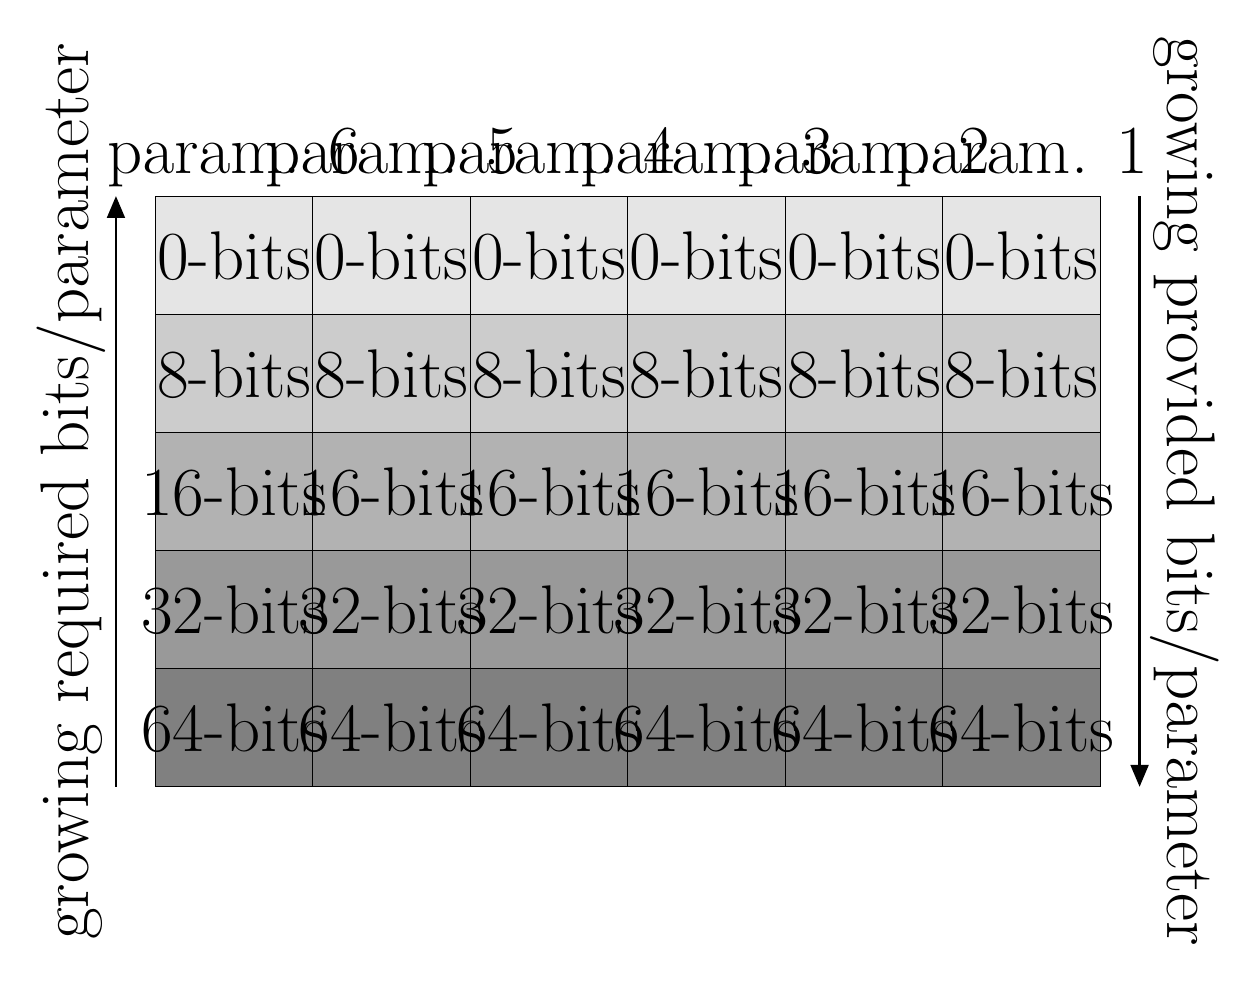
\begin{tikzpicture}

\fill[black!10!white] (0,7.5) rectangle (12,6);
\fill[black!20!white] (0,6) rectangle (12,4.5);
\fill[black!30!white] (0,4.5) rectangle (12,3);
\fill[black!40!white] (0,3) rectangle (12,1.5);
\fill[black!50!white] (0,1.5) rectangle (12,0);

\draw[-triangle 45, thick] (-0.5,0) -- node[sloped, anchor=center, above] {\Huge{growing required bits/parameter}} (-0.5,7.5);
\draw[-triangle 45, thick] (12.5,7.5) -- node[sloped, anchor=center, above] {\Huge{growing provided bits/parameter}} (12.5,0);

\draw (0,7.5)  --node[anchor=south] {\rot{\Huge{param. 6}}} (2,7.5);
\draw (2,7.5)  --node[anchor=south] {\rot{\Huge{param. 5}}} (4,7.5);
\draw (4,7.5)  --node[anchor=south] {\rot{\Huge{param. 4}}} (6,7.5);
\draw (6,7.5)  --node[anchor=south] {\rot{\Huge{param. 3}}} (8,7.5);
\draw (8,7.5)  --node[anchor=south] {\rot{\Huge{param. 2}}} (10,7.5);
\draw (10,7.5) --node[anchor=south] {\rot{\Huge{param. 1}}} (12,7.5);

\draw (0,7.5)  rectangle node[anchor=center] {\Huge{0-bits}} (2,6);
\draw (2,7.5)  rectangle node[anchor=center] {\Huge{0-bits}} (4,6);
\draw (4,7.5)  rectangle node[anchor=center] {\Huge{0-bits}} (6,6);
\draw (6,7.5)  rectangle node[anchor=center] {\Huge{0-bits}} (8,6);
\draw (8,7.5)  rectangle node[anchor=center] {\Huge{0-bits}} (10,6);
\draw (10,7.5) rectangle node[anchor=center] {\Huge{0-bits}} (12,6);

\draw (0,6)  rectangle node[anchor=center] {\Huge{8-bits}} (2,4.5);
\draw (2,6)  rectangle node[anchor=center] {\Huge{8-bits}} (4,4.5);
\draw (4,6)  rectangle node[anchor=center] {\Huge{8-bits}} (6,4.5);
\draw (6,6)  rectangle node[anchor=center] {\Huge{8-bits}} (8,4.5);
\draw (8,6)  rectangle node[anchor=center] {\Huge{8-bits}} (10,4.5);
\draw (10,6) rectangle node[anchor=center] {\Huge{8-bits}} (12,4.5);

\draw (0,4.5)  rectangle node[anchor=center] {\Huge{16-bits}} (2,3);
\draw (2,4.5)  rectangle node[anchor=center] {\Huge{16-bits}} (4,3);
\draw (4,4.5)  rectangle node[anchor=center] {\Huge{16-bits}} (6,3);
\draw (6,4.5)  rectangle node[anchor=center] {\Huge{16-bits}} (8,3);
\draw (8,4.5)  rectangle node[anchor=center] {\Huge{16-bits}} (10,3);
\draw (10,4.5) rectangle node[anchor=center] {\Huge{16-bits}} (12,3);

\draw (0,3)  rectangle node[anchor=center] {\Huge{32-bits}} (2,1.5);
\draw (2,3)  rectangle node[anchor=center] {\Huge{32-bits}} (4,1.5);
\draw (4,3)  rectangle node[anchor=center] {\Huge{32-bits}} (6,1.5);
\draw (6,3)  rectangle node[anchor=center] {\Huge{32-bits}} (8,1.5);
\draw (8,3)  rectangle node[anchor=center] {\Huge{32-bits}} (10,1.5);
\draw (10,3) rectangle node[anchor=center] {\Huge{32-bits}} (12,1.5);

\draw (0,1.5)  rectangle node[anchor=center] {\Huge{64-bits}} (2,0);
\draw (2,1.5)  rectangle node[anchor=center] {\Huge{64-bits}} (4,0);
\draw (4,1.5)  rectangle node[anchor=center] {\Huge{64-bits}} (6,0);
\draw (6,1.5)  rectangle node[anchor=center] {\Huge{64-bits}} (8,0);
\draw (8,1.5)  rectangle node[anchor=center] {\Huge{64-bits}} (10,0);
\draw (10,1.5) rectangle node[anchor=center] {\Huge{64-bits}} (12,0);
\end{tikzpicture}
}
\caption{The \emph{type} policy schema for callsites and calltargets. As is demonstrated here, when requiring width, one starts at the bottom and grows to the top, as it is always possible to accept more than one requires. The reverse is true for providing, as it is possible to accept less than provided.}
\label{fig:TYPEschema}
\end{figure}
As shown in Figure \ref{fig:TYPEschema}, our idea is to not simply classify callsites and calltargets based on the number of parameters they provide or request, but also on the parameter type. To simplify our approach, we use the width of the type and do not infer the actual type. As previously mentioned, there are 4 types of reading and writing accesses. Therefore, our set of possible types for parameters is $\texttt{TYPE} = \{64, 32, 16, 8, 0\}$; where 0 models the absence of a parameter. Since SystemV ABI specifies 6 registers as parameter holding registers, we classify our callsites and calltargets into $\texttt{TYPE}^6$. Similar to the policy of \texttt{TypeArmor}, we allow overestimations of callsites and underestimations of calltargets, however, on the level of types. Therefore, for a callsite $cs$ it is possible to call a calltarget $ct$, only if for each parameter of $ct$ the corresponding parameter of $cs$ is not smaller w.r.t. the width. This results in a finer-grained policy which is further restricting the possible pool of calltargets for each callsite.

%What we call the \emph{type} policy is the idea of not only relying on the parameter count but also on the parameter type. However, due to complexity reasons,
%we are restricting ourselves to the general purpose registers, which the SystemV ABI designates as parameter registers. Furthermore, we are not inferring 
%the actual type of the data but the wideness of the data stored in the register. The schema again is that we have calltargets requiring wideness and the
%callsite providing it as depicted in Figure \ref{fig:TYPEschema}.

%e are currently interested in x86-64 binaries, the registers we are looking at are 64-bit registers that can be accessed in four different ways:
%\textit{1)} the whole 64-bit of the register, meaning a wideness of 64,
%\textit{2)} the lower 32-bit of the register, meaning a wideness of 32,
%\textit{3)} the lower 16-bit of the register, meaning a wideness of 16, and
%\textit{4)} the lower 8-bit of the register, meaning a wideness of 8.

%Four of those registers can also directly access the higher 8-bit of the lower 16-bit of the register. For our purpose we register this access as a 16-bit access. 

%Based on this information,we can assign a register one of 5 possible types $\mathcal{T} = \{64, 32, 16, 8, 0\}$. We also included the type 0 to model the absence of data within a register. 
%Similar to the \emph{count} policy, we allow overestimation of types in callsites and underestimation of types in calltargets. However, the matching idea is different, 
%because as can we depict in Figure \ref{fig:TYPEschema}, the type of a calltarget and a callsite no longer depends solely on its parameter count, 
%each callsite and calltarget has its type from the set of $\mathcal{T}^6$, with the following comparison operator:
%$
%	u \leq_{type} v :\Longleftrightarrow  
%	\forall_{i = 0}^{5} {u_i \leq v_i} , \text {with } u, v \in \mathcal{T}^6
%$.

%Again we allow any callsite $cs$ call any calltarget $ct$, when it fulfills the requirement $ct \leq cs$. 
%The way we represent this is by letting the type for a calltarget parameter progress from 64-bit to 0-bit---if a calltarget requires a 32-bit value in its 1st parameter, it also should accept a 64-bit value from its callsite---and similarly we let the type for a callsite progress from 0-bit to 64-bit - If a callsite provides a 32-bit value in its 1st parameter it also provides a 16-bit, 8-bit and 0-bit to a calltarget. Now the advantage of the \emph{type} policy in comparison to the \emph{count} policy is that while our type comparison implies the count comparison, the other direction does not hold.
%Meaning, just having an equal or lesser number of parameters than a callsite, does no longer allow a calltarget being called there, thus restricting the number of calltargets per 
%callsite even further. A function that requires 64-bit in its first parameter, and 0-bit in all other parameters, would have been callable by a callsite providing 8-bit 
%in its first and second parameter when using the \emph{count} policy, however in the \emph{type} policy this is no longer possible. Thus, it should decrease the number of targets per bucket.


    
\subsection{Calltarget Analysis}
\label{section:calltargetanalysis}
For our policy, we need to classify calltargets according to the parameters they provide. Underestimations are allowed, however, overestimations shall not be permitted. For this purpose, we employ a customizable modified liveness analysis algorithm, which we will show first. We then present our versions for a~\emph{count} and a~\emph{type} based policy. Furthermore, we need to be aware of certain corner cases, which we will discuss at the end.

\subsubsection{Liveness Analysis}
A variable is alive before the execution of an instruction, if at least one of the originating paths performs a read access before any write access on that variable. If applied to a function, this calculates the variables that need to be alive at the beginning, as these are its parameters. We based Algorithm~\ref{alg:liveness} on the liveness analysis algorithm presented in Khedker~\textit{et al.}~\cite{khedker2009data}, which basically is a depth-first traversal of basic blocks. For customization, we rely on the implementation of several functions ($\mathcal{S}^\mathcal{L}$ is the set of possible register states depending on the specific liveness implementation):

$\texttt{merge\_v} : \mathcal{S}^\mathcal{L} \times \mathcal{S}^\mathcal{L} \mapsto \mathcal{S}^\mathcal{L}$, which describes how to merge a set of states resulting from several paths.

$\texttt{merge\_h} : \mathcal{P}(\mathcal{S}^\mathcal{L}) \mapsto \mathcal{S}^\mathcal{L}$, which describes how to merge the current state with the following state change.

$\texttt{analyze\_instr} : \texttt{INSTR} \mapsto \mathcal{S}^\mathcal{L}$, which calculates the state change that occurs due to the given instruction 

$\texttt{succ} : \texttt{INSTR}^* \mapsto \mathcal{P}(\texttt{INSTR}^*)$, which calculates the successors of the given block.

\begin{algorithm}[h!]
 	\SetAlgoLined
	\SetKwInOut{Input}{Input}
      \SetKwInOut{Output}{Output}
  \Input{block : $\texttt{INSTR}^*$}
        \Output{$\mathcal{S}^\mathcal{L}$}
        \BlankLine
	\SetKwProg{Fn}{Function }{ is}{end}
	\Fn{\texttt{analyze} (block : $\texttt{INSTR}^*$) : $\mathcal{S}^\mathcal{L}$}
	{
 	state = Bl                                                  \Comment*[r]{Initialize the state}
 	
 	\ForEach{inst $\in$ block}{
 	
 		state' = \texttt{analyze\_instr}(inst)	\Comment*[r]{Calculate changes}

		state = \texttt{merge\_h}(state, state')                     \Comment*[r]{Merge changes}
	}

	states = \{\}                                               \Comment*[r]{Set of surccessor states}
	
	blocks = \texttt{succ(block)}                                        \Comment*[r]{Get successors}
	
	\ForEach{block' $\in$ blocks} {
	
 		state' = \texttt{ analyze}(block') \Comment*[r]{Analyze successor }
 		
		states = states $\cup$ \{ state' \} \Comment*[r]{Add successor states}
	}

	state' = \texttt{merge\_h }(states)	\Comment*[r]{Merge successor states}

	\Return merge\_v(state, state')                             \Comment*[r]{Merge to final state}

	}
\caption{Basic block liveness analysis.}
\label{alg:liveness}
\end{algorithm}

In our specific case, the function \texttt{analyze\_instr} needs to also handle non-jump and non-fall-through successors, as these are not handled by DynInst. Essentially, there are four relevant cases: 1) If the current instruction is an indirect call or a direct call and the chosen implementation should not follow calls, 
then return a state where all registers are considered to be written before read. 2) If the current instruction is a direct call and the chosen implementation should follow calls, then we start an analysis of the target function and return its result. 3) If the instruction is a constant write (e.g., xor of two registers), then we remove the read portion before we return the decoded state. 4) In any other case, we simply return the decoded state. This leaves us with the two undefined merge functions and the undefined liveness state $\mathcal{S}^\mathcal{L}$. In the following two paragraphs we will present two implementation variants: first, similar to TypeArmor, a \emph{count} based policy and second our \emph{type} based policy.

\subsubsection{Required Parameter Count} 
To implement the \emph{count} policy, we only need a coarse representation of the state of one register, thus we use the same representation as TypeArmor: 1) $W$ represents write before read access, 2) $R$ represents read before write access, and 3) $C$ represents the absence of access. This gives us the $S^\mathcal{L} = \{ C, R, W \}$ as register state, which translates to the register super state $\mathcal{S}^\mathcal{L} = (S^\mathcal{L})^{16}$. We implement \texttt{merge\_v} in such a way that a state within a superstate is only updated if the corresponding register has yet to be accessed, as represented by $C$. Our reasoning is that the first access is the relevant one to determine read before write.

%TODO  \texttt{merge\_h} (depends on numbers)

The index of highest parameter register based on the used call convention that has the state R is considered to be the number of parameters a function at least requires to be prepared by a callsite.

%
%This leaves us with the two merge functions remaining undefined and we will leave the implementation of these and the interpretation of the  liveness state $\mathcal{S}^\mathcal{L}$ into parameters up to the following subsections.
%
%\textbf{Required Parameter Count.}
%\label{subsection:requiredparamcount}
%To implement the \emph{count} policy, we only need a coarse representation of the state of one register, thus we use the same representation as TypeArmor:
%\textit{1)} $W$ represents write before read access,
%\textit{2)} $R$ represents read before write access, and
%\textit{3)} $C$ represents the absence of access.
%
%This gives us the following register state $S^\mathcal{L} = \{ C, R, W \}$ which translates to the register super state $\mathcal{S}^\mathcal{L} = (S^\mathcal{L})^{16}$.
%We are only interested in the first occurrence of a $R$ or $W$ within one path, as following reads or writes do not give us more information. 
%Therefore, our vertical merge function ($merge\_v$) behaves in the following way that only when the first given state is $C$, 
%is the return value the second state and in all other cases it will return the first state.
%
%\begin{align}
%merge\_v^{r} (cur, delta) &= \left\{
%  \begin{array}{lr}
%     delta & cur = C \\
%     cur & otherwise
%  \end{array}
%\right. \\Liveness analysis of a 
%merge\_v (cur, delta) &= (s'_0, ... s'_15) \text { with } s'_j = merge\_v^{r}(cur_j, delta_j)
%\end{align}

%Our horizontal merge($merge\_h$) function is a simple pairwise combination of the given set of states, 
%which are then combined with a union like operator with $W$ preceding $R$ preceding $C$.
%\begin{align}
%merge\_h(\{s\}) &= s\\
%merge\_h(\{s\} \cup s') &= s \circ merge\_h(s')
%\end{align}

%
%We have three viable possibilities for our combination operator $\circ$, depicted in Table \ref{fig:COUNTlivenessmapping}, which all give priority to $W$:
%\begin{itemize}
%\item [$\bigsqcap^{\mathcal{L}}$] is what we call the destructive combination operator, as it returns W on any mismatch.
%\item [$\bigcap^{\mathcal{L}}$] is what we call the intersection operator, as it returns C, when combining C and R, similar to an intersection.
%\item [$\bigcup^{\mathcal{L}}$] is what we call the union operator, as it returns R, when combining C and R similar to a union.
%\end{itemize}


\newcolumntype{?}{!{\vrule width 1pt}}
%
%\begin{table}
%
%% \centering
%\resizebox{\columnwidth}{!}{%Liveness analysis of a 
%\begin{tabular}{c?c|c|c}
%$\bigsqcap^{\mathcal{L}}$ & C & R & W\\
%\Xhline{1pt}
%C & C & W & W\\
%\hline
%R & W & R & W\\
%\hline
%W & W & W & W
%\end{tabular}
%\begin{tabular}{c?c|c|c}
%$\bigcap^{\mathcal{L}}$  & C & R & W\\
%\Xhline{1pt}
%C & C & C & W\\
%\hline
%R & C & R{todo} & W\\
%\hline
%W & W & W & W
%\end{tabular}
%\begin{tabular}{c?c|c|c}
%$\bigcup^{\mathcal{L}}$  & C & R & W\\
%\Xhline{1pt}
%C & C & R & W\\
%\hline
%R & R & R & W\\
%\hline
%W & W & W & W
%\end{tabular}}
%\caption{Different mappings for combining two liveness state values in horizontal matching for the \emph{count} policy.}
%
%\label{fig:COUNTlivenessmapping}
%\end{table}

%The index of highest parameter register based on the used call convention that has the state R is considered to be the number of parameters a function at least requires to be prepared by a callsite.

\subsubsection{Required Parameter Wideness}
\label{subsection:requiredparamwideness}
To implement the \emph{type} policy, we need a finer representation of the state of one register:
\textit{1)} $W$ represents write before read access,
\textit{2)} $r8, r16, r32, r64$ represents read before write access with 8-, 16-, 32-, 64-bit width, and
\textit{3)} $C$ represents the absence of access.
%\begin{enumerate}
%\item Was the register written to before its value could be read ? \\ We represent this with the state $W$.
%\item How much was read from the register before its value was overwritten? \\ We represent this with the states $\{ r8, r16, r32, r64 \}$ 
%using $R$ as a placeholder for arbitrary reads.
%\item Did neither read nor write access occur for the register ? \\ We represent this with the state $C$.
%\end{enumerate}
This gives us the following $S^\mathcal{L} = \{ C, r8, r16, r32, r64, W \}$ register state which translates to the register super state 
$\mathcal{S}^\mathcal{L} = (S^\mathcal{L})^{16}$.
%Now, we assume that unless the instructions we are looking at does discard the value it is reading (\texttt{xor rax rax} would be such 
%an instruction that we call const\_write) that reading does precede the writing withing one instruction.
As there could be more than one read of a register before it is written, we might be interested in more than just the first occurrence of a write or read on a path. 
To permit this, we allow our merge operations to also return the value $RW$, which represents the existence of both read and write access and then can use $W$ with the functionality of an end marker.
% We arrive therefore at three possible vertical merge functions:
%\begin{itemize}
%	\item The same vertical merge operator as used in the \emph{count} policy, which only gives us the first non $C$ state ($merge\_v^{r}$).
%	\item A vertical merge operator that conceptually intersects all read accesses along a path until the first write occurs ($merge\_v^{i}$).
%	\item A vertical merge operator that conceptually calculates the union of all read accesses along a path until the first write occurs ($merge\_v^{u}$).
%\end{itemize}
Therefore, our vertical merge operator conceptually intersects all read accesses along a path until the first write 
occurs ($merge\_v^{i}$). In any other case, it behaves like the previously mentioned vertical merge function.
%Our horizontal merge function is a simple pairwise combination of the given set of states:
%\begin{align}
%merge\_h(\{s\}) &= s\\
%merge\_h(\{s\} \cup s') &= s \circ merge\_h(s')
%\end{align}
Our horizontal merge($merge\_h$) function is again a simple pairwise combination of the given set of states, which are then combined with a union-like operator with $W$ preceding $WR$ preceding $R$ preceding $C$. Unless one side is $W$, read accesses are combined in such a way that always the higher one is chosen.

%The results of our experiments with the implementation of calltarget classification gave presented us with essentially one possible candidate
%that we can base our horizontal merge function on, namely the union operator with an analysis function that follows into direct calls. The 
%basic schema of the merging is depicted in \ref{tbl:TYPECTunion} and it essentially behaves as if it was the union operator (when both states
%are set, the higher one is chosen). However, we have to account for W being used as an end marker, which is why we added mapping for RW, 
%which is essentially that. 
%
%\begin{table}[h]
%\centering
%% \resizebox{\columnwidth}{!}{%
%\begin{tabular}{c?c|c|c|c}
%$\bigcup^{\mathcal{L}}$  & C & R & W & RW\\
%\Xhline{1pt}
%C & C & R & W & RW\\
%\hline
%R & R & $\text{R}^{\cup}$ & W & $\text{R}^{\cup}$W\\
%\hline
%W & W & W & W & W\\Liveness analysis of a 
%\hline
%RW & RW & $\text{R}^{\cup}$W & W & RW\\
%\end{tabular}
%% }
%\caption{The union mapping operator for liveness in the \emph{type} policy.}
%\label{tbl:TYPECTunion}
%\end{table}

\subsubsection{Variadic Functions}
\label{subsection:variadicfunctions}

\begin{figure}[thp] % the figure provides the caption
\centering          % which should be centered
\begin{tabular}{c}  % the tabular makes the listing as small as possible and centers it
\footnotesize
\begin{lstlisting}
00000000004222f0 <make_cmd>:
 4222f0:push   %r15
 4222f2:push   %r14
 4222f4:push   %rbx
 4222f5:sub    $0xd0,%rsp
 4222fc:mov    %esi,%r15d
 4222ff:mov    %rdi,%\begin{figure}[!h]
 422302:test   %al,%al
 422304:je     42233d <make_cmd+0x4d>
 422306:movaps %xmm0,0x50(%rsp)
 42230b:movaps %xmm1,0x60(%rsp)
 422310:movaps %xmm2,0x70(%rsp)
 422315:movaps %xmm3,0x80(%rsp)
 42231d:movaps %xmm4,0x90(%rsp)
 422325:movaps %xmm5,0xa0(%rsp)
 42232d:movaps %xmm6,0xb0(%rsp)
 422335:movaps %xmm7,0xc0(%rsp)
 42233d:mov    %r9,0x48(%rsp)
 422342:mov    %r8,0x40(%rsp)
 422347:mov    %rcx,0x38(%rsp)
 42234c:mov    %rdx,0x30(%rsp)
 422351:mov    $0x50,%esi
 422356:mov    %r14,%rdi
 422359:callq  409430 <pcalloc>
\end{lstlisting}
\end{tabular}
\caption{ASM code of the \texttt{make\_cmd} function with optimize level O2, which has a variadic parameter list.}
\label{fig:asmvariadic}
\end{figure}

Variadic functions are special functions in C/C++ that have a basic set of parameters, 
which they always require and a variadic set of parameters, which as the name suggests 
may vary. A prominent example of this would be the $printf$ function, which is used 
to output text to $stdout$.
This type of functions allows for an easier processing of parameters where
usually all potential variadic parameters are moved into a contiguous block of memory, 
as can be observed in the assembly depicted in Figure \ref{fig:asmvariadic}.
Our analysis interprets that as a read access on all parameters and thus,
we arrive at a potentially problematic overestimation. 

Our solution to this problem is to find these spurious reads and ignore them. A compiler will implement this type of operation very 
similar for all cases, thus we can achieve our desired outcome using the following steps:
\textit{1)} we search for (what we call) the xmm-passthrough block, which entirely consists of moving values of registers \texttt{xmm0} to \texttt{xmm7} into contiguous memory, % (in our case basic block [\texttt{0x422306}, \texttt{0x42233d} [ ).
\textit{2)} we look at the predecessor of the xmm-passthrough block, which we call the entry block (in our case basic block %[\texttt{0x4222f0},\texttt{0x4222f2} [ )
Check if the successors of the entry block consist of the xmm-passthrough block and the successor of the 
xmm-passthrough block, which we call the param-passthrough block, and
%(in our case basic block [\texttt{0x42233d}Liveness analysis of a , \texttt{0x42235e} [ )
\textit{3)} We look at the param-passthrough block and set all instructions that move the value of a parameter register into memory to be ignored. %(in our case the instructions \texttt{0x42233d}, \texttt{0x422342}, \texttt{0x422347} and \texttt{0x42234c})

\subsubsection{Ignoring Reads} When one instruction writes and reads a register at the same time, we give the read access precedence, however, there are exceptions (also mentioned in TypeArmor, however, we expand slightly on that):
\textit{1)} \texttt{xor \%rax, \%rax} is the first obvious scenario, as it will always result in \texttt{\%rax} holding the value 0,
\textit{2)} \texttt{sub \%rax, \%rax} is probably the next scenario, as it results in \texttt{\%rax} also holding the value 0, and
\textit{3)} \texttt{sbb \%rax, \%rax} is also relevant, however, it will not result in a constant value and based on the current state might either result in \texttt{\%rax} holding the value 0 or 1.

\begin{algorithm}[!ht]
	\SetAlgoLined
	\SetKwInOut{Input}{Input}
        \SetKwInOut{Output}{Output}
        \Input{basic block}
        \Output{$\mathcal{S}^\mathcal{R}$}
        \BlankLine
	\SetKwProg{Fn}{Function}{ is}{end}
	\Fn{analyze(block : BasicBlock) : $\mathcal{S}^\mathcal{R}$}
	{
 	state = Bl                                   \Comment*[r]{Some comment}
 	
 	\ForEach{inst $\in$ reversed(block)}{
 	
 		state' = analyze\_instr(inst)        \Comment*[r]{Some comment}
 		
		state = merge\_v(state, state')      \Comment*[r]{Some comment}
	}

	states = \{\}                                \Comment*[r]{Some comment}
	
	blocks = pred(block)                         \Comment*[r]{Some comment}
	
	\ForEach{block' $\in$ blocks} {
	
 		state' = analyze(block')             \Comment*[r]{Some comment}
 		
		states = states $\cup$ \{ state' \}  \Comment*[r]{Some comment}
	}

	state' = merge\_h (states)                   \Comment*[r]{Some comment}

	\Return merge\_v(state, state')              \Comment*[r]{Some comment}

	}
\caption{Basic block reaching definition analysis.}
\label{alg:reaching}
\end{algorithm}

\subsection{Callsite Analysis}
\label{section:callsiteanalysis}
For either \emph{count} or \emph{type} policy to work, we need to arrive at an overestimation of the provided parameters by any indirect callsite existing within the targeted binary. We will employ a modified version of reaching analysis that tracks registers instead of variables to generate the needed overestimation. As our algorithm will be customizable, we look at the required merge functions to implement the \emph{count} and \emph{type} policies. 

\subsubsection{Reaching Definitions}
\label{subsection:reachindefinitionstheory}
An assignment of a value to a variable is a reaching definition at the end of a block $n$, if that definition is present within at 
least one path from start to the end of the block $n$ without being overwritten by another value assignment to the same variable. 
We employ reaching definitions analysis, because we are looking for the parameters a callsite provides. This essentially 
requires the last known set of definitions that reach the actual call instruction within the parameter registers.

%The book~\cite{khedker2009data} defines reaching definition analysis on blocks in the following manner:
%\begin{subequations}
%\label{eq:reachingbasedef}
%\begin{align}
%In_n &:= \left\{
%  \begin{array}{lr}
%    Bl & \text{n is start block}\\
%    \underset{p \in pred(n)}{\bigcup} Out_p & \text{otherwise}
%  \end{array}
%\right. \label{eq:reachingbasedefInt}\\
%Out_n &:= (In_n - Kill_n) \cup Gen_n \label{eq:reachingbasedefOut}
%\end{align}
%\end{subequations}
%$Bl$ is the default state at the start of a path of execution and in our case reaching that state would mean that we do not 
%know whether a value has been provided for the variable and therefore we assume that one has been provided, reaching an 
%overestimation. The set $Kill_n$ describes all definitions that are removed within this block, meaning that the value of 
%a variable has been overwritten. The set $Gen_n$ describes the new definitions that have been provided by the block $n$, 
%meaning that the value of a variable has been assigned. Considering this, we can assume that $Gen_n \subseteq Kill_n$, 
%as we can always create new definitions, but not simply remove definitions without assigning a new value to the variable.


%
%
%However, we cannot use reaching definition analysis as is, because the analysis is again based on potentially unbound 
%variable sets, while we are restricted to a finite number of registers and states. This time however, the analysis provides us with an overestimation, 
%we however, want to get a result as close as possible so we again want to customize merge functions. Furthermore, we have to define how 
%to interpret the changes occuring withing one block based on the the change caused by its instructions. Considering this, w, we 
%arrive at algorithm \ref{alg:reaching} to compute the liveness state at the start of a basic block.
Previous work~\cite{khedker2009data} provides a reaching definition analysis on blocks, which we use to arrive at the algorithm depicted in Algorithm~\ref{alg:reaching} to compute the liveness state at the start of a basic block. We apply the reaching analysis at each indirect callsite directly before each call instruction.

This algorithm relies on various functions that can be used to configure its behavior. We need to define the 
function $merge\_v$, which describes how to compound the state change of the current instruction and the current state, 
the function $merge\_h$, which describes how to merge the states of several paths, the instruction analysis function
$analyze\_instr$. Note, that the function $pred$, which retrieves all possible predecessors of a block has not been implemented by us, because we rely on the DynInst instrumentation framework to achieve the following.
\vspace{-.3cm}
\begin{subequations}
\label{eq:livenesscustom}
\begin{align}
merge\_v &: \mathcal{S}^\mathcal{R} \times \mathcal{S}^\mathcal{R} \mapsto \mathcal{S}^\mathcal{L}\\
merge\_h &: \mathcal{P}(\mathcal{S}^\mathcal{R}) \mapsto \mathcal{S}^\mathcal{R}\\
analyze\_instr &: \mathcal {I} \mapsto \mathcal{S}^\mathcal{R} \\
pred &: \mathcal{I} \mapsto \mathcal{P}(\mathcal{I})
\end{align}
\end{subequations}
\vspace{-.8cm}

The $analyze\_instr$ function calculates the effect of an instruction and is the heart of the analyze function. It will also 
handle non-jump and non-fall-through successors, as these are not handled by DynInst in our case. We essentially have three cases that we handle:
\textit{1)} If the instruction is an indirect call or a direct call but we chose not to follow calls, then return a state where all trashed are considered written,
\textit{2)} If the instruction is a direct call and we chose to follow calls, then we spawn a new analysis and return its result, and
%\item if the instruction is a constant write (\textit{e.g.,} xor of two registers) then we remove the read portion before we return the decoded state
\textit{3)} In all other cases, we simply return the decoded state.

This leaves us with the two merge functions remaining undefined and we will leave the implementation of these and the interpretation of the liveness state $\mathcal{S}^\mathcal{L}$ into parameters up to the following subsections.

%We have yet to define the functions $merge\_v$, which describes how to compound a function and the outgoing state, the function $merge\_h$, which describes how to merge the states of several paths and the function $pred$, which essentially gives us the predecessors of the current instruction. To prevent cycles we keep track of the instructions visited within the current path and omit any instruction on the current path from the result of $pred$. These functions, the reaching state $\mathcal{S}^\mathcal{R}$  and its interpretation into parameters will be defined in the following subsections.
%
%
%\subsection{Backward Graph Traversal}
%\label{subsection:backwardgraphtraversal}

\subsubsection{Provided Parameter Count}
\label{subsection:providedparamcount}
To implement the \emph{count} policy, we only need a coarse representation of the state of one register, thus we use the same representation as TypeArmor:
\textit{1)} $T$ represents a trashed register,
\textit{2)} $S$ represents a set register (written to), and
\textit{3)} $U$ represents an untouched register.
This gives us the following $S^\mathcal{L} = \{ T, S, U \}$  register state which translates to the register super state $\mathcal{S}^\mathcal{R} = (S^\mathcal{R})^{16}$.

We are only interested in the first occurrence of a $S$ or $T$ within one path, as following reads or writes do not give us more information. Therefore, our vertical merge function ($merge\_v$) behaves in the following way: only when the first given state is $U$, is the return value the second state and in all other cases it will return the first state.
%
%We are only interested in the first occurrence of a S or T within one path, as following reads or writes do not give us more information.
%Therefore, we can define our vertical merge function in the following way:
%\begin{align}
%merge\_v^{r} (cur, delta) &= \left\{
%  \begin{array}{lr}
%     delta & cur = U \\
%     cur & otherwise
%  \end{array}
%\right. \\
%merge\_v (cur, delta) &= (s'_0, ... s'_15) \text { with } s'_j = merge\_v^{r}(cur_j, delta_j)
%\end{align}


Our horizontal merge($merge\_h$) function is a simple pairwise combination of the given set of states, which are then combined with a union like operator with $T$ preceding $S$ preceding $U$.
%
%Our horizontal merge function is a simple pairwise combination of the given set of states:
%\begin{align}
%merge\_h(\{s\}) &= s\\
%merge\_h(\{s\} \cup s') &= s \circ merge\_h(s')
%\end{align}
%
%We have four viable possibilities for our combination operator $\circ$, depicted in table \ref{fig:COUNTreachingmapping}, which all (except one) give priority to $T$:
%\begin{itemize}
%\item [$\bigsqcap^{\mathcal{R}}$] is what we call the destructive combination operator, as it returns T on any mismatch.
%\item [$\bigcap^{\mathcal{R}}$] is what we call the intersection operator, as it returns U, when combining U and S, similar to an intersection.
%\item [$\bigcup^{\mathcal{R}}$] is what we call the union operator, as it returns S, when combining U and S similar to a union.
%\item [$\bigsqcup^{\mathcal{R}}$] is what we call the true union operator, as it gives S precedence over everything and returns T or 
%U only when both sides are T or U being more inclusive than a union.
%\end{itemize}

\newcolumntype{?}{!{\vrule width 1pt}}
%
%\begin{table}
%% \centering
%{
%\resizebox{\columnwidth}{!}{%
%\begin{tabular}{c?c|c|c}
%$\bigsqcap^{\mathcal{R}}$ & U & S & T\\
%\Xhline{1pt}
%U & U & T & T\\
%\hline
%S & T & S & T\\
%\hline
%T & T & T & T
%\end{tabular}
%\begin{tabular}{c?c|c|c}
%$\bigcap^{\mathcal{R}}$  & U & S & T\\
%\Xhline{1pt}
%U & U & U & T\\
%\hline
%S & U & S & T\\
%\hline
%T & T & T & T
%\end{tabular}
%\begin{tabular}{c?c|c|c}
%$\bigcup^{\mathcal{R}}$  & U & S & T\\
%\Xhline{1pt}
%U & U & S & T\\
%\hline
%S & S & S & T\\
%\hline
%T & T & T & T
%\end{tabular}
%\begin{tabular}{c?c|c|c}
%$\bigsqcup^{\mathcal{R}}$  & U & S & T\\
%\Xhline{1pt}
%U & U & S & T\\
%\hline
%S & S & S & S\\
%\hline
%T & T & S & T
%\end{tabular}}
%}
%
%\caption{Different mappings for combining two reaching state values in horizontal matching for the \emph{count} policy.}
%
%\label{fig:COUNTreachingmapping}
%\end{table}

The index of the highest parameter register based on the used call convention that has the state S is considered to be the number of parameters a callsite at most prepares.

\subsubsection{Provided Parameter Width}
\label{subsection:providedparamwideness}
In order to implement the \emph{type} policy, we need a finer representation of the state of one register:
\textit{1)} $T$ represents a trashed register,
\textit{2)} $s8, s16, s32, s64 S$ represents a set register with  8-, 16-, 32-, 64-bit width, and
\textit{3)} $U$ represents an untouched register.
%\begin{itemize}
%\item Was the register value trashed ? \\ We represent this with the state T.
%\item Was the register written to and how much ? \\ We represent this with the states $\{ s64, s32, s16, s8 \}$ using S as a placeholder for arbitrary writes.
%\item Was the register neither trashed nor written to ? \\ We represent this with the state U.
%\end{itemize}
This gives us the following $S^\mathcal{L} = \{ T, s64, s32, s16, s8, U \}$ register state which translates to the register 
super state $\mathcal{S}^\mathcal{R} = (S^\mathcal{R})^{16}$.

Again, we are only interested in the first occurrence of a state that is not $U$ in a path, as following reads or writes do not give us more information. Therefore, we can use the same vertical merge function as for the \emph{count} policy, which is essentially a pass-through until the first non $U$ state.

Our horizontal merge($merge\_h$) function is a simple pairwise combination of the given set of states, which are then combined with a union like operator with $T$ preceding $S$ preceding $U$. When both states are set, we pick the higher one.

%
%Our horizontal merge function is again a simple pairwise combination of the given set of states:
%\begin{align}
%merge\_h(\{s\}) &= s\\
%merge\_h(\{s\} \cup s') &= s \circ merge\_h(s')
%\end{align}
%
%However, we have different possibilities regarding the merge operator. Experiments with our implementations for callsite 
%classification in the \emph{count} policy have given us the following results:
%\begin{itemize}
%\item The best candidate to minimize the problematic matches is the union operator without following direct calls.
%\item The best candidate to maximize precision is the intersection operator with following direct calls.
%\end{itemize}
%
%We therefore arrive at three viable possibilities for our combination operator $\circ$, depicted in table \ref{fig:TYPEreachingmapping}, 
%which all (except one) give priority to $T$:
%\begin{itemize}
%\item [$\bigcap^{\mathcal{R}}$] is what we call the intersection operator, as it returns U, when combining U and S, similar to an 
%intersection furthermore we also calculate the intersection of states when both states are set 
%(the lower of the two is returned).
%\item [$\bigsqcap^{\mathcal{R}}$] is what we call the half intersection operator, as it returns U, when combining U and S, 
%similar to an intersection but we calculate the union of states when both states are set (the higher of the two is returned).
%\item [$\bigcup^{\mathcal{R}}$] is what we call the union operator, as it returns S, when combining U and S similar to a union
%furthermore we calculate the union of states when both states are set (the higher of the two is returned).
%\end{itemize}
%
%\begin{table}
%
%% \centering
%\resizebox{\columnwidth}{!}{%
%\begin{tabular}{c?c|c|c}
%$\bigcap^{\mathcal{R}}$  & U & S & T\\
%\Xhline{1pt}
%U & U & U & T\\
%\hline
%S & U & $\text{S}^{\cap{}{}}$ & T\\
%\hline
%T & T & T & T
%\end{tabular}
%\begin{tabular}{c?c|c|c}
%$\bigsqcap^{\mathcal{R}}$  & U & S & T\\
%\Xhline{1pt}
%U & U & U & T\\
%\hline
%S & U & $\text{S}^{\cup{}{}}$ & T\\
%\hline
%T & T & T & T
%\end{tabular}
%\begin{tabular}{c?c|c|c}
%$\bigcup^{\mathcal{R}}$  & U & S & T\\
%\Xhline{1pt}
%U & U & S & T\\
%\hline
%S & S & $\text{S}^{\cup{}{}}$ & T\\
%\hline
%T & T & T & T
%\end{tabular}}
%
%\caption{Different mappings for combining two reaching state values in horizontal matching for the \emph{type} policy.}
%\label{fig:TYPEreachingmapping}
%\end{table}

Our experiments with this implementation showed two problems regarding the provided width detection. Parameter lists with \textit{holes} and address width underestimation, furthermore register extension instructions are also cause of problems. To reduce runtime, we also restricted the maximum path depth to 10 blocks.

\paragraph{Parameter Lists with \textit{Holes}.} This refers to parameter lists that show one or more \texttt{void} parameters between start to the last actual parameter. These are not existent in actual code, but our analysis has the possibility of generating them through the merge operations. An example would be the following: 
A parameter list of $(64, 0, 64, 0, 0, 0)$ is concluded, although the actual parameter list might be $(64, 32, 64, 0, 0, 0)$. While the trailing 0s are 
what we expect, the 0 at the second parameter position will cause trouble, because it is an underestimation at the single parameter level, which we need to avoid.
Our solution is to scan our reaching analysis result for these holes and replace them with the wideness $64$, causing a (possible) overestimation.

\paragraph{Address Width Unterestimation.} This refers to the issue that while in the callsite a constant value of 32-bit is written to a register, the calltarget uses the whole 64-bit register. This can occur when pointers are passed from the callsite to the calltarget. Specifically this happens 
when pointers to memory inside the \texttt{.bss}, \texttt{.data} or \texttt{.rodata} section of the binary are passed.
Our solution is to enhance our instruction analysis to watch out for constant writes. In case a 32-bit constant value write is detected, we check if the
value is an address within the \texttt{.bss}, \texttt{.data} or \texttt{.rodata} section of the binary. If this is the case, we simply return a write access of 64-bit 
instead of 32-bit. This is not problematic, because we are looking for an overestimation of parameter wideness.
It should be noted that the same problem can arise when a constant write causes the value 0 to be written to a 32-bit register. We use the same solution
and set the width to 64-bit instead of 32-bit.
%
%\subsection{Address Taken Analysis}
%\label{section:addresstakenanalysis}
%As of now, we use the maximum available set of calltargets---the set of all function entry basic blocks---as input for our algorithm. 
%To restrict the number of calltargets per callsite even further, we explored the possibility of incorporating an address taken analysis
%into our application. We base our theory on the paper by Zhang \textit{et al.}~\cite{mingwei:sekar}, which introduced various types of taken
%addresses. An address is considered to be taken, when it is loaded into memory or a register.
%
%\textbf{Address Taken Targets.}
%Based on the notions of \cite{mingwei:sekar}, which classified taken addresses into several types of indirect control flow targets,
%we only chose { Code Pointer Constants (CK)} and discarded the others:
%\begin{itemize}
%
%\item { Code Pointer Constants (CK)} are addresses that are calculated during the compilation of the binary and point within
%the possible range of addresses in the current module or to instruction boundaries. We are however, only interested in addresses
%that directly point to an entry basic block of a function, as these are the only valid targets for any callsite.
%
%\item { Computed code pointers (CC)} are the result of simple pointer arithmetic, however, these are only used for intra-procedural jumps. 
%We rely on DynInst to resolve those and only focus on indirect callsites, therefore these are of no interest to us.
%
%\item{ Exception handling addresses (EH)} are used to handle exceptions within C++ functions and are modeled as jumps within the function. 
%These are therefore within the normal control flow that we rely on DynInst to resolve for us.
%
%\item{ Exported function addresses (ES)} are essentially functions that point outside of our current module (usually to dynamically 
%linked libraries) and are implemented as jumps, which are of no concern to us, because our analysis is only concerned about the current object.
%
%\item { Return addresses (RA)}, which are the addresses next to a call instruction, are also of no interest to us, because we only 
%implement forward { control flow integrity}.
%\end{itemize}
%
%\textbf{Binary Analysis.}
%Our approach of identifying taken addresses consists of two steps: First, we iterate over the raw binary content of data sections. Second,
%we iterate over all functions within the disassembled binary. We rely on DynInst to provide us with the boundaries of the sections inside
%the binary and in case of shared libraries with the needed translation to current memory addresses:
%
%\begin{itemize}
%\item We look at three different data sections of the binary, which could possibly contain taken addresses: the .data, .rodata and .dynsym
%sections. As \cite{mingwei:sekar} proposed, we slide a four byte window over the data within those sections and look for addresses that
%point to function entry blocks. However, we are looking at x64 binaries therefore we additionally use an eight byte window. In case of 
%shared libraries, we need to let DynInst translate the raw address, we extracted, so we can perform the function check.
%
%\item We specifically look for instructions that load a constant value into a register or memory, and again check whether the address 
%points to the entry block of a function.
%\end{itemize}

%\section{Runtime Enforcement}
%\label{section:runtimeenforcement}
%
%\subsection{Calltarget Annotation}
%\label{subsection:patchingschema}
%
%\subsection{Callsite Instrumentation}
%\label{subsection:patchingschema}



\section{Implementation}
\label{chapter:Implementation}

We implemented \textsc{TypeShield} as a module pass for the \textit{di-opt} environment pass provided by the DynInst~\cite{bernat:dyninst} 
instrumentation framework (v.9.2.0). However, converting the pass to a standalone executable is also possible, as we do not rely on 
an extended set of DynInst features except for the pass abstraction. We currently restricted our analysis and instrumentation to x86-64 
bit elf binaries using the SystemV call convention, because the DynInst library does not yet support the
Windows platform. However, there is ongoing work to allow DynInst to work with Windows binaries as well. We focused on the SystemV call 
convention as most C/C++ compilers on Linux implement this ABI, however, we encapsulated most ABI-dependent behavior, so it should be 
possible to implement other ABIs with relative ease. Therefore, we deem it possible to implement \textsc{TypeShield} for the Windows 
platform in the near future, as we do not use any other platform-dependent APIs. We developed the core part of our pass in an instruction
analyzer, which relies on the DynamoRIO~\cite{dynamorio:drmemory} library (v.6.6.1) to decode single instructions and provide access to
its information. The analyzer is then used to implement our version of the reaching and liveness analysis (similar to PathArmor~\cite{veen:typearmor}), 
which can be customized with relative ease, as we allow for arbitrary path merging functions. However, we implemented the three basic versions as 
follows: destructive, intersection and union. To accomplish this, we patched the DynInst library in order to allow for local annotation of 
calltargets with arbitrary information, leveraging its relocation schema, which relies on the basic block abstraction. We implemented a 
Clang/LLVM (v.4.0.0, trunk 283889) pass used for 
collecting ground truth data in order to measure the quality and performance of our tool. The ground truth data is then used to verify 
the output of our tool for several test targets. This is accomplished with the help of our Python-based evaluation and test environment. 
In total, we implemented \textsc{TypeShield} in 5556 lines of code (LOC) of C++ code, our Clang/LLVM pass in 392 LOC
of C++ code and our test environment in 3005 Python LOC. 



\section{Evaluation}
\label{chapter:Evaluation}
We evaluated \textsc{TypeShield} by instrumenting various open source applications and analyzing the results. 
We used the two ftp server applications \textit{vsftpd} (v.1.1.0) and \textit{proftpd} (v.1.3.3), the two http server 
applications \textit{postgresql} (v.9.0.10) and \textit{mysql} (v.5.1.65), the memory cache application \textit{memcached} (v.1.4.20) 
and the \textit{node.js} server application (v.0.12.5). We chose these applications, which are a subset of the 
applications also used by the TypeAmor~\cite{veen:typearmor} to allow for later comparison.
In our evaluation we addressed the following research questions:
\begin{itemize}
 \item \textbf{RQ1:} How precise is \textsc{TypeShield}? (\cref{section:typeshieldprecision})

 \item \textbf{RQ2:} What level of security does \textsc{TypeShield} offer? (\cref{section:typeshieldeffectiveness})

 \item \textbf{RQ3:} What is the runtime overhead of \textsc{TypeShield}? (\cref{section:typeshieldoverheadperformance})

 \item \textbf{RQ4:} What is the instrumentation overhead of \textsc{TypeShield}? (\cref{section:typeshieldoverheadinstrumentation})

 \item \textbf{RQ5:} Is our tool better than other tools? (\cref{RQ5: Is TypeShield better than other tools?})
\end{itemize}
\textbf{Comparison Method.} As we do not have access (we requested the Authors several times to provide access to the source code) to the source code of TypeAmor, we implemented two modes in \textsc{TypeShield}. 
The first mode of our tool is an similar implementation of the \textit{count} 
policy described by TypeArmor. The second mode is our implementation of the \textit{type} policy on
top of our \textit{count} policy implementation. 
%
%\textbf{Experimental Setup.} We setup our environment within a VirtualBox (version 5.0.26r) instance, which runs Kubuntu 16.04 LTS (Linux Kernel
%version 4.4.0) and has access to 3GB of RAM and 4 of 8 provided hardware threads (Intel i7-4170HQ @ 2.50 GHz).

\subsection{RQ1: Precision of \textsc{TypeShield}}
\label{section:typeshieldprecision}
\todo[inline]{In this section we need just one or two Table similar to what TypeArmor contains, first we need to define the fields which make most sense.}

To measure the precision of \textsc{TypeShield}, we need to compare the classification of call-sites and call-targets as is given by our tool to
some sort of ground truth for our test targets. We generate this ground truth by compiling our test targets using a custom compiled Clang/LLVM
compiler (v.4.0.0 trunk 283889) with a MachineFunction pass inside the x86 code generation implementation of LLVM. We essentially 
collect three data points for each call-site/call-target from our LLVM-pass:
\textit{1)} The point of origination, which is either the name of the call-target or the name of the function the call-site resides in.
\textit{2)} The return type that is either expected by the call-site or provided by the call-target.
\textit{3)} The parameter list that is provided by the call-site or expected by the call-target, which discards the variadic argument list.

However, before we can proceed to measure the quality and precision of \textsc{TypeShield}'s classification of call-targets and call-sites
using our ground truth, we need to evaluate the quality and applicability of the ground truth, we collected.

\subsubsection{Quality and Applicability of Ground Truth}
\label{subsection:typeshieldprecision}
To assess the applicability of our collected ground truth, we essentially need to assess the structural compatibility of our two datasets.
First, we take a look at the comparability of call-targets and second, we take a look at the compatibility of call-sites. The results are depcited in Table \ref{tbl:matchingquality}.

\begin{table}[h!]
\resizebox{\columnwidth}{!}{
	\begin{tabular}{l|r|r|r|r|r|r}%
	\toprule
	\multicolumn{1}{c}{\bfseries O2} & \multicolumn{3}{c|}{ {\bfseries call-targets}} & \multicolumn{3}{c}{{\bfseries call-sites} }\\
	\bfseries Target & match & Clang miss &  tool miss &  match & Clang miss & tool miss% specify table head
	\\\midrule
	\csvreader[before filter=\ifthenelse{\equal{\csvcoli}{geomean}}{\csvfilterreject}{\csvfilteraccept},  late after line=\\, late after last line=\\\midrule]{csvs/matching.O2.csv}{
		%1=\target, 2=\opt, 3=\fns, 4=\fnsnotClang, 5=\fnsnotpadyn, 6=\ats, 7=\atnotClang, 8=\atnotpadyn, 9=\cscount, 10=\csClang, 11=\cspadyn
	}
	{\csvcoli & \csvcoliii & \csvcoliv (\csvcolv \% )& \csvcolvi (\csvcolvii \% )& \csvcolxiii & \csvcolxiv  (\csvcolxv) & \csvcolxvi   (\csvcolvii) }% specify your coloumns here

	\csvreader[before filter=\ifthenelse{\equal{\csvcoli}{geomean}}{\csvfilteraccept}{\csvfilterreject},  late after line=\\, late after last line=\\\bottomrule]{csvs/matching.O2.csv}{
		%1=\target, 2=\opt, 3=\fns, 4=\fnsnotClang, 5=\fnsnotpadyn, 6=\ats, 7=\atnotClang, 8=\atnotpadyn, 9=\cscount, 10=\csClang, 11=\cspadyn
	}
	{\csvcoli & \csvcoliii & \csvcoliv \ (\csvcolv \% )& \csvcolvi \ (\csvcolvii \% )& \csvcolxiii & \csvcolxiv \ (\csvcolxv) & \csvcolxvi \ (\csvcolvii) }% specify your coloumns here
    	\end{tabular}
    	
    	}
%     	}
	\caption {Table shows the quality of structural matching provided by our automated verify and test environment, 
	regarding call-sites and call-targets when compiling with optimization level O2. The label Clang miss 
	denotes elements not found in the data-set of the Clang/LLVM pass. The label tool miss denotes elements not found in the data-set of \textsc{TypeShield}.}
	\label{tbl:matchingquality}
\end{table}

\textbf{Call-targets.} The obvious choice for structural comparison regarding call-targets is their name, as these are simply functions. 
First, we have to remove internal functions from our data-sets like the \texttt{\_init} or \texttt{\_fini} functions, which are of no consequence for us. 
Furthermore, while C functions can simply be matched by their name as they are unique through the binary, the same cannot be said about the 
language C++. One of the key differences between C and C++ is function overloading, which allows to define several functions with the same name, as 
long as they differ in namespace or parameter type. As LLVM does not know about either concept, the Clang compiler needs to generate unique names. 
The method used for unique name generation is called mangling and composes the actual name of the function, its the return type, its name-space and the 
types of its parameter list. We therefore need to reverse this process and then compare the fully typed names.
Table \ref{tbl:matchingquality} shows three data points regarding call-targets for the optimization level O2:
\textit{1)}  The number of comparable call-targets that are found in both datasets
\textit{2)}  Clang miss: The number of call-targets that are found by \textsc{TypeShield} but not by our Clang/LLVM pass
\textit{3)}  tool miss: The number of call-targets that are found by our Clang/LLVM pass but not by \textsc{TypeShield}

The problematic column is the Clang miss column, as these might indicate problems with \textsc{TypeShield}. These numbers are relatively low (below 1\%) with only node showing a significant higher value than the rest (around 1.6\%). The column labeled tool miss lists 
higher numbers, however these are of no real concern to us, as our ground truth pass possibly collects more data: All source files used during the 
compilation of our test-targets are incorporated into our ground truth. The compilation might generate more than one binary and therefore not 
necessary all source files are used for our test-target.

Considering this, we can safely state that our structural matching between ground truth and \textsc{TypeShield} regarding call-targets is nearly
perfect (above 98\%)\\


\textbf{Call-sites.} While our structural matching of call-targets is rather simple, the matter of matching callsites is more complex. Our tool can provide accurate addressing of call-sites within the binary. However, Clang/LLVM does not have such capabilities in its intermediate representation (IR). Furthermore the IR is not the final representation within the compiler, as the IR is transformed into a machine-based representation (MR), which is the again optimized. Although we can read information regarding paramters from the IR, it is not possible with the MR. Therefore we attach that data directly after the conversion from IR to MR and read that data at the end of the compilation. To not unneccessarily pollute our dataset, we only considered call-targets, which have been found in both datasets. 
The table \ref{tbl:matchingquality} shows three data points regarding call-sites for the optimization level O2:
\textit{1)} The number of comparable call-sites that are found in both datasets.
\textit{2)} Clang miss: The number of call-sites that are discarded from the dataset of \textsc{TypeShield}.
\textit{3)} tool miss: The number of call-sites that are discarded from the dataset of our Clang/LLVM pass.

Both columns (Clang miss and tool miss) show a relatively low number of problems (<0.5\%), therefore we can also safely state that our structural matching between ground truth and \textsc{TypeShield} regarding call-sites is also nearly perfect (above 99\%)

\subsubsection{Classification Precision (\textit{count})}
\label{subsection:typeshieldcountprecision}

We measured two data points per target, the number and ratio of perfect classifications and the number and ratio of problematic classifications, which in the case of calltargets refers to overestimations and in case of callsites refers to underestimations. The results are depicted in Table \ref{tbl:precisionCOUNT}.
\begin{table}[h!]
\resizebox{\columnwidth}{!}{
	\begin{tabular}{l|r|r|r|r|r|r}%

	\toprule
	\multicolumn{1}{c}{\bfseries O2} & \multicolumn{3}{c}{\bfseries Call-targets} & \multicolumn{3}{c}{\bfseries Call-sites}\\
	
	\bfseries Target & \#  &  perfect &  problem & \# & perfect &  problem % specify table head
	\\\midrule
	\csvreader[before filter=\ifthenelse{\equal{\csvcolii}{geomean}}{\csvfilterreject}{\csvfilteraccept}, late after line=\\, late after last line=\\\midrule]{csvs/classification_comp.sources_union_follow.O2.csv}{
		%1=opt,2=target,3=cs,4=cs args,5=perfect,6=cs args,7=problem,8 = cs non-void ,9=correct,10 = cs non-void, 11=problem,12 = ct, 13 = ct args, 14=perfect, 15 = ct args, 16=problem, 17 = ct void, 18=correct, 19=ct void, 20=problem
}
	{\csvcolii  &  \csvcolxii & \csvcolxiii \ (\csvcolxiv \%) & \csvcolxv \ (\csvcolxvi \%) & \csvcoliii & \csvcoliv \ (\csvcolv \%) & \csvcolvi \ (\csvcolvii\%)}% specify your coloumns here

	\csvreader[before filter=\ifthenelse{\equal{\csvcolii}{geomean}}{\csvfilteraccept}{\csvfilterreject}, late after line=\\, late after last line=\\\bottomrule]{csvs/classification_comp.sources_union_follow.O2.csv}{
		%1=opt,2=target,3=cs,4=cs args,5=perfect,6=cs args,7=problem,8 = cs non-void ,9=correct,10 = cs non-void, 11=problem,12 = ct, 13 = ct args, 14=perfect, 15 = ct args, 16=problem, 17 = ct void, 18=correct, 19=ct void, 20=problem
}
	{\csvcolii  &  \csvcolxii & \csvcolxiii \ (\csvcolxiv \%) & \csvcolxv \ (\csvcolxvi \%) & \csvcoliii & \csvcoliv \ (\csvcolv \%) & \csvcolvi \ (\csvcolvii\%)}% specify your coloumns here
    	\end{tabular}

}
		\caption {The results for analysis using the \textit{count} policy on the O2 optimization level.}
		\label{tbl:precisionCOUNT}
\end{table}~\\
\textbf{Experiment Setup (Call-targets).} Union combination operator with an $analyze$ function that follows into occurring direct calls.
\textbf{Results (Call-targets).} The problem rate is under 0.01\%, as there are only two testtargets, that exhibit a problematic classification. The rate of perfect classification is in general over 80\% with mysql as an exception (73.85\%) resulting in a geometric mean of 86.86\%.
\textbf{Experiment Setup (Call-sites)} Union combination operator with an $analyze$ function that does not follow into occurring direct calls while relying on a backward inter-procedural analysis.
\textbf{Results (Call-sites).} The problem rate is under 0.01\%, as there is only one testtarget, that exhibit a problematic classification. The rate of perfect classification is in general over 60\% with nginx (48.49\%) and node (56.34\%) as an exception resulting in a geometric mean of 71.97\%.


\subsubsection{Classification Precision (\textit{type})}
\label{subsection:typeshieldcountprecision}

We measured two data points per testtarget, the number and ratio of perfect classifications and the number and ratio of problematic classifications, which in the case of calltargets refers to overestimations and in case of callsites refers to underestimations. The results are depicted in Table \ref{tbl:precisionTYPE}.
\begin{table}[h!]
\resizebox{\columnwidth}{!}{
	\begin{tabular}{l|r|r|r|r|r|r}%

	\toprule
	\multicolumn{1}{c}{\bfseries O2} & \multicolumn{3}{c}{\bfseries Call-targets} & \multicolumn{3}{c}{\bfseries Call-sites}\\
	
	\bfseries Target & \#  &  perfect &  problem & \# & perfect &  problem % specify table head
	\\\midrule
	\csvreader[before filter=\ifthenelse{\equal{\csvcolii}{geomean}}{\csvfilterreject}{\csvfilteraccept},  late after line=\\, late after last line=\\\midrule]{csvs/classification_comp2.type_exp6.O2.csv}{
		%1=opt,2=target,3=cs,4=cs args,5=perfect,6=cs args,7=problem,8 = cs non-void ,9=correct,10 = cs non-void, 11=problem,12 = ct, 13 = ct args, 14=perfect, 15 = ct args, 16=problem, 17 = ct void, 18=correct, 19=ct void, 20=problem
}
	{\csvcolii  &  \csvcolxii & \csvcolxiii \ (\csvcolxiv \%) & \csvcolxv \ (\csvcolxvi \%) & \csvcoliii & \csvcoliv \ (\csvcolv \%) & \csvcolvi \ (\csvcolvii\%)}% specify your coloumns here

	\csvreader[before filter=\ifthenelse{\equal{\csvcolii}{geomean}}{\csvfilteraccept}{\csvfilterreject},  late after line=\\, late after last line=\\\bottomrule]{csvs/classification_comp2.type_exp6.O2.csv}{
		%1=opt,2=target,3=cs,4=cs args,5=perfect,6=cs args,7=problem,8 = cs non-void ,9=correct,10 = cs non-void, 11=problem,12 = ct, 13 = ct args, 14=perfect, 15 = ct args, 16=problem, 17 = ct void, 18=correct, 19=ct void, 20=problem
}
	{\csvcolii  &  \csvcolxii & \csvcolxiii \ (\csvcolxiv \%) & \csvcolxv \ (\csvcolxvi \%) & \csvcoliii & \csvcoliv \ (\csvcolv \%) & \csvcolvi \ (\csvcolvii\%)}% specify your coloumns here
    	\end{tabular}

}
		\caption {The results for analysis using the \textit{type} policy on the O2 optimization level.}
		\label{tbl:precisionTYPE}
\end{table}~\\
\textbf{Experiment Setup (Call-targets).} Union combination operator with an $analyze$ function that does follow into occurring direct calls  and a vertical merge that intersects all reads until the first write.
\textbf{Results (Call-targets).} For half of the set, the problem rate is under 1\% and for the other half it is not above 10\%, resulting in a geomean of 1.92\%. The rate of perfect classification is in general over 70\% with nginx (69.38\%) and mysql (63.16\%)  resulting in a geometric mean of 77.15\%.
\textbf{Experiment Setup (Call-sites).} Union combination operator with an $analyze$ function that does not follow into occurring direct calls while relying on a backward inter-procedural analysis.
\textbf{Results (Call-sites).} For two thirds of the set, the problem rate is under 2\% and for last third it is not above 10\%, resulting in a geomean of 1.38\%.  The rate of perfect classification is in general over 50\% with node (44.76\%) as an exception resulting in a geometric mean of 68.35\%.


%
%
%Efficiency
%
%
\subsection{RQ2: Security Level of \textsc{TypeShield}}
\label{section:typeshieldeffectiveness}
\todo[inline]{In this section we need just one or two Table similar to what TypeArmor contains, 
first we need to define the fields which make most sense.}

\begin{table*}[htbp!]
\begin{center}
 \resizebox{2\columnwidth}{!}{
	\begin{tabular}{l|r|rcl|r|rcl|r|rcl|r|rcl|r}%

	\toprule
	\multicolumn{1}{c}{\bfseries O2} & \multicolumn{1}{c}{\bfseries AT} & \multicolumn{4}{c}{\bfseries \textit{count}*} & \multicolumn{4}{c}{\bfseries \textit{count}} & \multicolumn{4}{c}{\bfseries \textit{type}*} & \multicolumn{4}{c}{\bfseries \textit{type}}\\
	
	\bfseries Target && \multicolumn{3}{c}{ limit (mean $\pm$ $\sigma$)} & median & \multicolumn{3}{c}{ limit (mean $\pm$ $\sigma$)} & median & \multicolumn{3}{c}{ limit (mean $\pm$ $\sigma$)} & median & \multicolumn{3}{c}{ limit (mean $\pm$ $\sigma$)} & median  % specify table head
	\\\midrule
	\csvreader[before filter=\ifthenelse{\equal{\csvcolii}{geomean}}{\csvfilterreject}{\csvfilteraccept},  late after line=\\, late after last line=\\\midrule]{csvs/policy_compare_at.O2.csv}{
	%1=opt,2=target,3=at,4=count safe avg,5=count safe sig,6=count safe median,7=count prec avg,8=count prec sig,9=count prec median,10=count* avg,11=count* sig,12=count* median,13=type safe avg,14=type safe sig,15=type safe median,16=type prec avg,17=type prec sig,18=type prec median,19=type* avg,20=type* sig,21=type* median
 }
	{\csvcolii  &  \csvcoliii & \csvcolx & $\pm$ & \csvcolxi & \csvcolxii & \csvcolvii & $\pm$ & \csvcolviii& \csvcolix& \csvcolxix & $\pm$ & \csvcolxx& \csvcolxxi & \csvcolxvi & $\pm$ & \csvcolxvii& \csvcolxviii }% specify your coloumns here

	\csvreader[before filter=\ifthenelse{\equal{\csvcolii}{geomean}}{\csvfilteraccept}{\csvfilterreject},  late after line=\\, late after last line=\\\bottomrule]{csvs/policy_compare_at.O2.csv}{
	%1=opt,2=target,3=at,4=count safe avg,5=count safe sig,6=count safe median,7=count prec avg,8=count prec sig,9=count prec median,10=count* avg,11=count* sig,12=count* median,13=type safe avg,14=type safe sig,15=type safe median,16=type prec avg,17=type prec sig,18=type prec median,19=type* avg,20=type* sig,21=type* median
 }
	{\csvcolii  &  \csvcoliii & \csvcolx & $\pm$ & \csvcolxi & \csvcolxii & \csvcolvii & $\pm$ & \csvcolviii& \csvcolix& \csvcolxix & $\pm$ & \csvcolxx& \csvcolxxi & \csvcolxvi & $\pm$ & \csvcolxvii& \csvcolxviii }% specify your coloumns here

    	\end{tabular}

}
	\caption {The results of comparing our implementation results with the theoretical limits for the different restriction policies combined with an address taken analysis for optimization level O2.}
	\label{tbl:policycompat}
\end{center}
\end{table*}

We are now going to evaluate the effectiveness of \textsc{TypeShield} leveraging the result of several experiment runs: First we are going to establish a baseline using the data 
collected from our Clang/LLVM pass, which are the theoretical limits our implementation can reach for both the \textit{count} and the \textit{type} schema. Second we are going to evaluate the effectiveness of our \textit{count} 
policy and third we are going to evaluate the effectiveness of our \textit{type} policy. For each series we collected three data points per test target, the average number of call-targets per call-site, the standard deviation $\sigma$ and the median. The results are depicted in table \ref{tbl:policycompat}. 

\subsubsection{Theoretical Limits.}
\label{subsection:theoreticallimit}
We explore the theoretical limits regarding the effectiveness of the \textit{count} and \textit{type} policies by relying on the collected ground truth data, essentially assuming perfect classification.
\textbf{Experiment Setup.} Based on the type information collected by our Clang/LLVM pass, we conducted two experiment series.
We derived the available number of call-targets for each call-site based on the collected ground truth applying the \textit{count} and \textit{type} schema

\textbf{Results.}
\textit{1)} The theoretical limit of the \textit{count*} schema has a geometric mean of 233 possible call-targets, which is 16.48\% of the geometric mean of total available 
call-targets, and
\textit{2)} The theoretical limit of the \textit{type*} schema has a geometric mean of 210 possible call-targets, which is 14.86\% of the geometric mean of total available
call-targets.

When compared, the theoretical limit of the \textit{type} policy allows about 10\% less available call-targets in the geomean in O2 than the limit of the \textit{count} policy.

\subsubsection{Reduction achieved by \textsc{TypeShield}}
\label{subsection:typeshieldvslimitcount}
\textbf{Experiment Setup.} We setup our two experiment series based on our previous evaluations regarding the classification precision for the \textit{count} and the \textit{type} policy.

\textbf{Results.}
\textit{1)}  The \textit{count} schema has a geometric mean of 315 possible call-targets, which is 22.29\% of the geometric mean of total available 
call-targets. This is 35.19\% more than the theoretical limit of available call-targets per call-site, and
\textit{2)}  The \textit{type} schema has a geometric mean of 290 possible call-targets, which is 20.52\% of the geometric mean of total available
call-targets. This is 38.09\% more than the theoretical limit of available call-targets per call-site.

When compared, our implementation of the \textit{type} policy allows about 7.93\% less available call-targets in the geomean in O2 than our implementation of the \textit{type} policy.


%\begin{table}[h!]
%\resizebox{.4\textwidth}{!}{
%	\begin{tabular}{l|c|rcl|c|rcl|c}%
%
%	\toprule
%	\multicolumn{1}{c}{\bfseries O2} & \multicolumn{1}{c}{\bfseries AT} & \multicolumn{4}{c}{\bfseries \textit{count} safe} & \multicolumn{4}{c}{\bfseries \textit{count} prec}\\
%	
%	\bfseries Target && \multicolumn{3}{c}{ limit (mean $\pm$ $\sigma$)} & median & \multicolumn{3}{c}{ limit (mean $\pm$ $\sigma$)} & median  % specify table head
%	\\\midrule
%	\csvreader[ late after line=\\, late after last line=\\\midrule]{../MA_Pictures/policy_compare_at.O2.csv}{
%	%1=opt,2=target,3=at,4=count safe avg,5=count safe sig,6=count safe median,7=count prec avg,8=count prec sig,9=count prec median,10=count* avg,11=count* sig,12=count* median,13=type safe avg,14=type safe sig,15=type safe median,16=type prec avg,17=type prec sig,18=type prec median,19=type* avg,20=type* sig,21=type* median
% }
%	{\csvcolii  &  \csvcoliii & \csvcoliv & $\pm$ & \csvcolv & \csvcolvi & \csvcolvii & $\pm$ & \csvcolviii& \csvcolix}% specify your coloumns here
%
%    	\end{tabular}
%}
%		\caption {The results of comparing \textit{count} safe and precision implementation restricted using an address taken analysis throughout different optimizations.}
%		\label{tbl:policycompatcount}
%\end{table}
%
%\begin{table}[h!]
%\resizebox{.4\textwidth}{!}{
%	\begin{tabular}{l|c|rcl|c|rcl|c}%
%
%	\toprule
%	\multicolumn{1}{c}{\bfseries O2} & \multicolumn{1}{c}{\bfseries AT} & \multicolumn{4}{c}{\bfseries \textit{type} safe} & \multicolumn{4}{c}{\bfseries \textit{type} prec}\\
%	
%	\bfseries Target && \multicolumn{3}{c}{ limit (mean $\pm$ $\sigma$)} & median & \multicolumn{3}{c}{ limit (mean $\pm$ $\sigma$)} & median  % specify table head
%	\\\midrule
%	\csvreader[ late after line=\\, late after last line=\\\midrule]{../MA_Pictures/policy_compare_at.O2.csv}{
%	%1=opt,2=target,3=at,4=count safe avg,5=count safe sig,6=count safe median,7=count prec avg,8=count prec sig,9=count prec median,10=count* avg,11=count* sig,12=count* median,13=type safe avg,14=type safe sig,15=type safe median,16=type prec avg,17=type prec sig,18=type prec median,19=type* avg,20=type* sig,21=type* median
% }
%	{\csvcolii  &  \csvcoliii & \csvcolxiii & $\pm$ & \csvcolxiv & \csvcolxv & \csvcolxvi & $\pm$ & \csvcolxvii& \csvcolxviii}% specify your coloumns here
%
%    	\end{tabular}
%}
%		\caption {The results of comparing \textit{type} safe and precision implementation restricted using an address taken analysis throughout different optimizations.}
%		\label{tbl:policycompattype}
%\end{table}

%
%\newpage
%\section{Security Analysis of \textsc{TypeShield}}
%\label{section:typeshieldsecurityanalysis}
%
%In this section, we discuss how effective \textsc{TypeShield} is 
%stopping advance code-reuse attacks (CRAs).
%Patching Policies
%Two types of diagrams. Table 5 from TypeArmor and a CDF to compare param count and param type. (baseline)
%here we put the CDF graphs from. There is no accurate security metrics to asses the security level of the enforced policy.
%
%
%
%\begin{table}
%\centering
%\resizebox{0.8\textwidth}{!}{
%	\begin{tabular}{l|c|c|c|c|c|c|c|c|c}%
%	\toprule
%	\multicolumn{1}{c}{\bfseries O0} & \multicolumn{1}{c}{} & \multicolumn{8}{|c}{ {\bfseries parameters}} \\
%	\bfseries Target & \bfseries \#CS & \bfseries -x & \bfseries +0 & \bfseries +1 & \bfseries +2 & \bfseries +3 & \bfseries +4 & \bfseries +5 & \bfseries +6 % specify table head
%	\\\midrule
%	\csvreader[ late after line=\\, late after last line=\\\midrule]{../MA_Pictures/classification_cs.O0.csv}{
%		%1=target,2=opt,3=cs,4=problems,5=+0,6=+1,7=+2,8=+3,9=+4,10=+5,11=+6,12=non-void-ok,13=non-void-problem
%	}
%	{\csvcoli & \csvcoliii & \csvcoliv & \csvcolv & \csvcolvi & \csvcolvii & \csvcolviii & \csvcolix & \csvcolx & \csvcolxi }% specify your coloumns here
%
%	\multicolumn{1}{c}{\bfseries O1}
%	\\\midrule
%	\csvreader[ late after line=\\, late after last line=\\\midrule]{../MA_Pictures/classification_cs.O1.csv}{
%		%1=target,2=opt,3=cs,4=problems,5=+0,6=+1,7=+2,8=+3,9=+4,10=+5,11=+6,12=non-void-ok,13=non-void-problem
%	}
%	{\csvcoli & \csvcoliii & \csvcoliv & \csvcolv & \csvcolvi & \csvcolvii & \csvcolviii & \csvcolix & \csvcolx & \csvcolxi}% specify your coloumns here
%
%	\multicolumn{1}{c}{\bfseries O2}
%	\\\midrule
%	\csvreader[ late after line=\\, late after last line=\\\midrule]{../MA_Pictures/classification_cs.O2.csv}{
%		%1=target,2=opt,3=cs,4=problems,5=+0,6=+1,7=+2,8=+3,9=+4,10=+5,11=+6,12=non-void-ok,13=non-void-problem
%	}
%	{\csvcoli & \csvcoliii & \csvcoliv & \csvcolv & \csvcolvi & \csvcolvii & \csvcolviii & \csvcolix & \csvcolx & \csvcolxi}% specify your coloumns here
%
%	\multicolumn{1}{c}{\bfseries O3}
%	\\\midrule
%	\csvreader[ late after line=\\, late after last line=\\\bottomrule]{../MA_Pictures/classification_cs.O3.csv}{
%		%1=target,2=opt,3=cs,4=problems,5=+0,6=+1,7=+2,8=+3,9=+4,10=+5,11=+6,12=non-void-ok,13=non-void-problem
%	}
%	{\csvcoli & \csvcoliii & \csvcoliv & \csvcolv & \csvcolvi & \csvcolvii & \csvcolviii & \csvcolix & \csvcolx & \csvcolxi}% specify your coloumns here
%
%
%    	\end{tabular}
%	}
%		\caption {Table shows the overestimation of the parameter count in matched callsites occurring in our precision focussed implementation of the \textit{count} policy, with -x denoting problematic callsites, when compiling with optimization levels O0 through O3}
%	\label{tbl:baselinecs}
%\end{table}
%
%\begin{figure}
%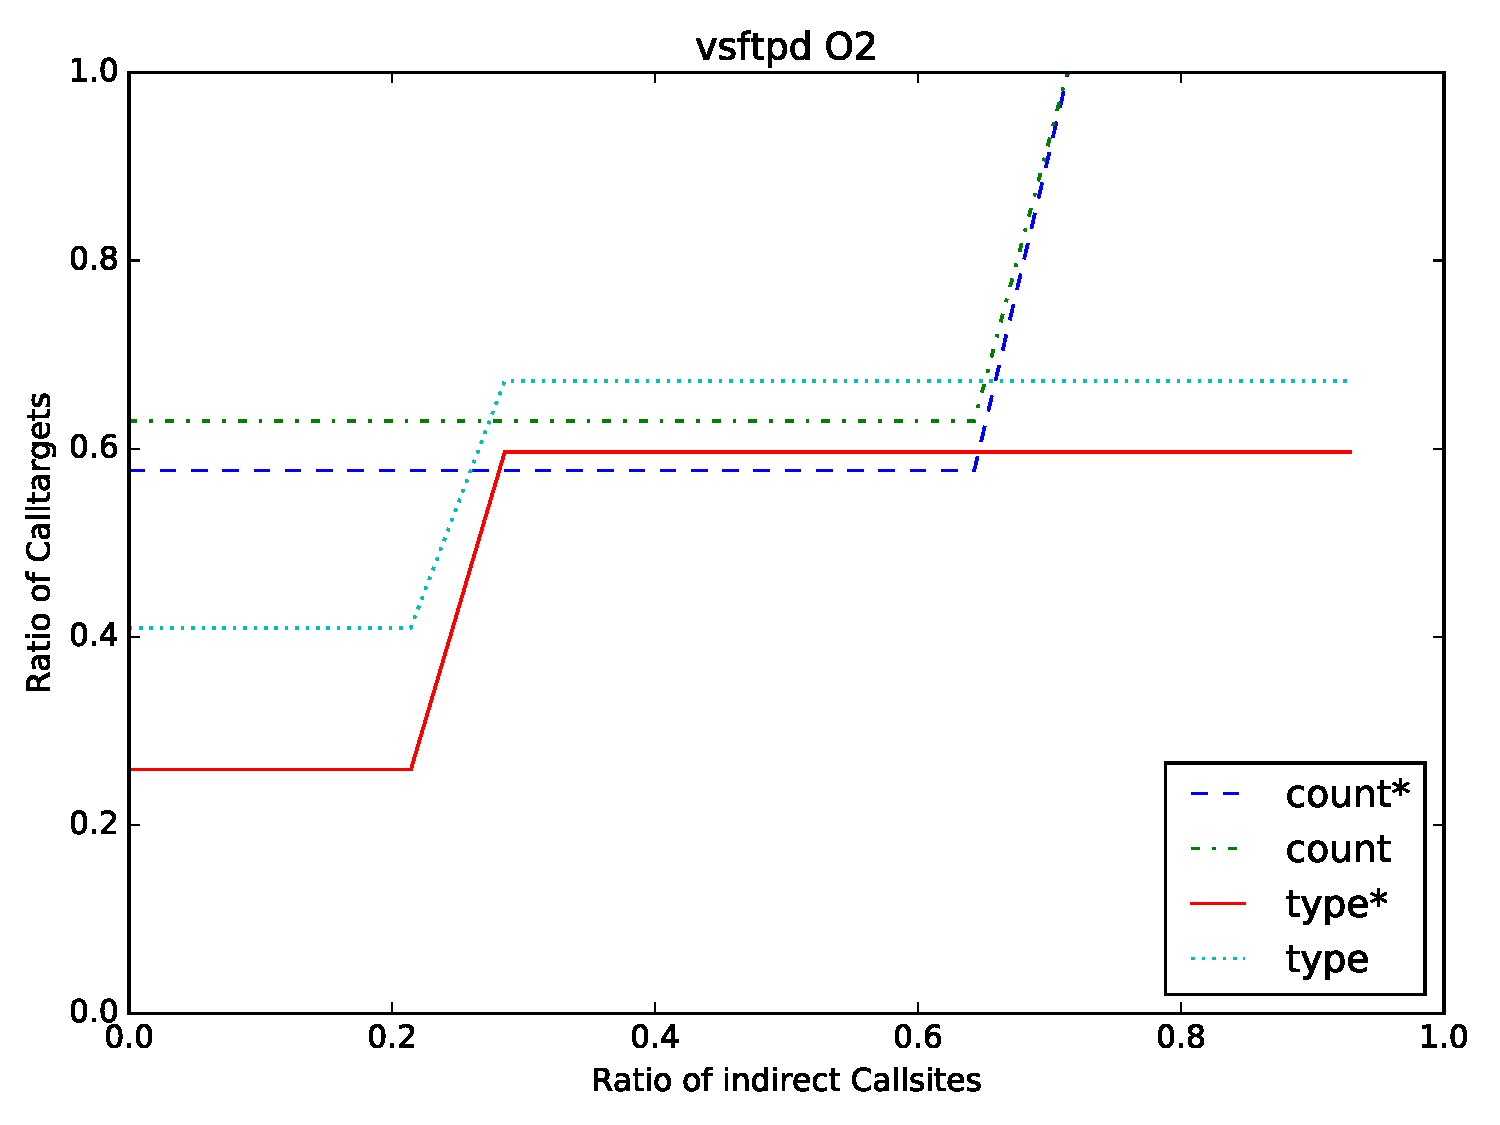
\includegraphics[width=0.5\textwidth]{../MA_Pictures/vsftpd.pdf}
%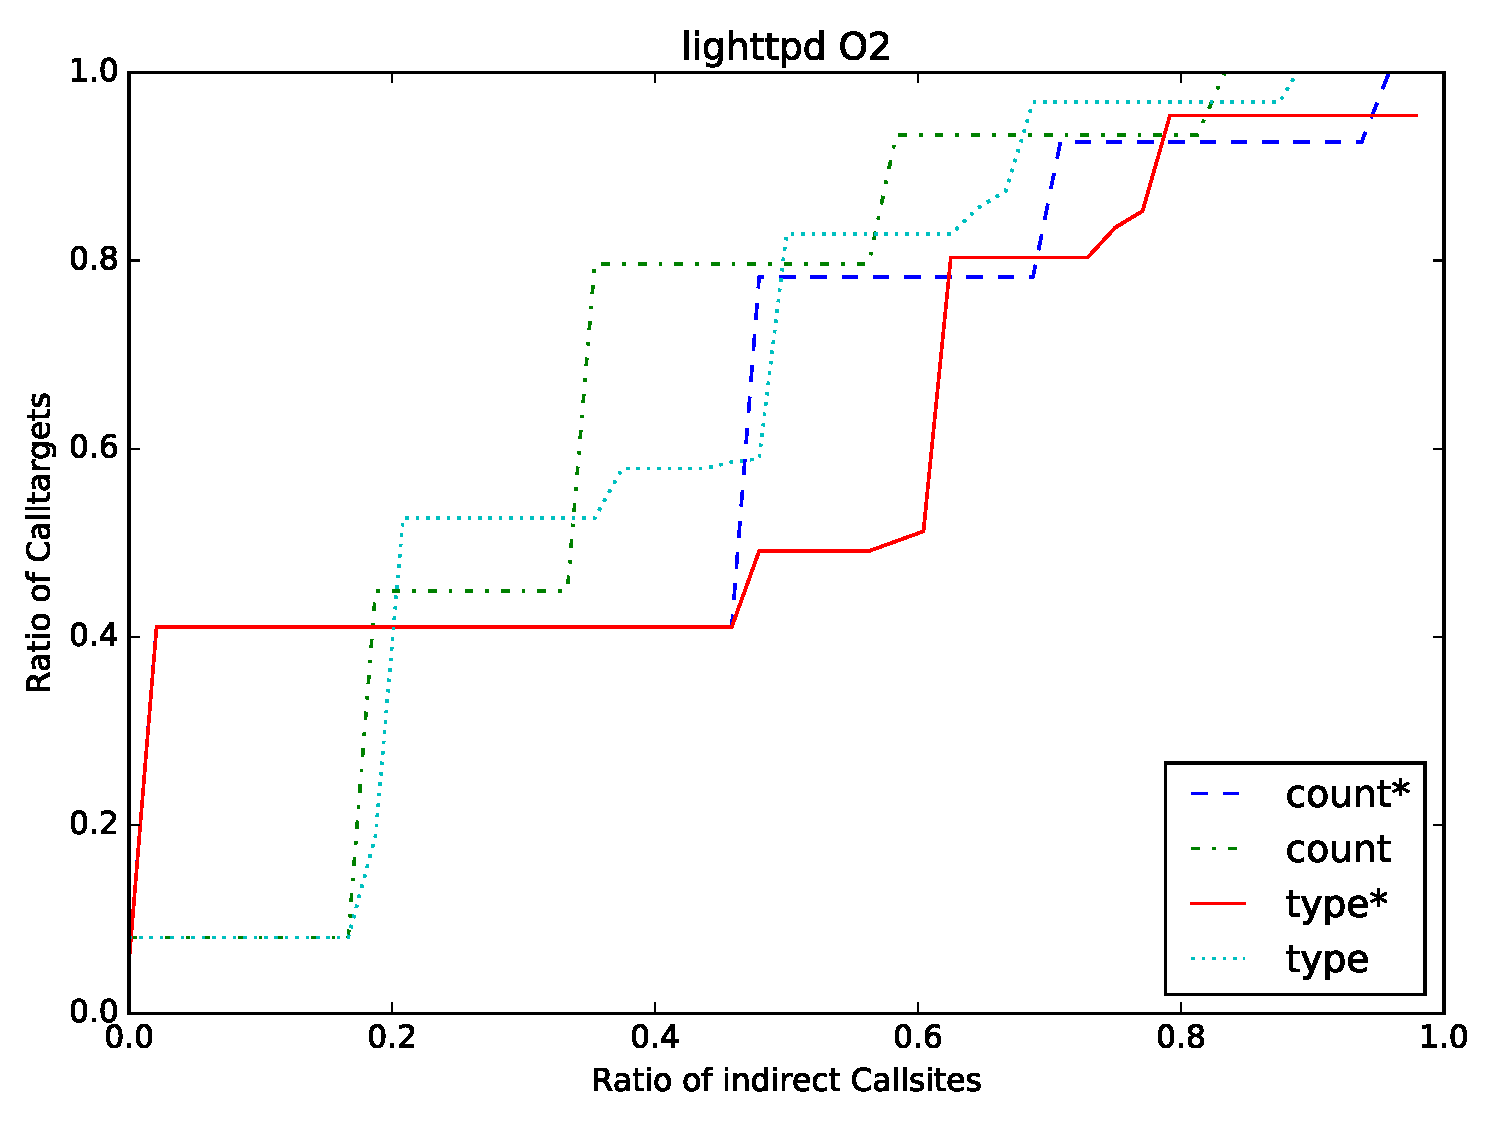
\includegraphics[width=0.5\textwidth]{../MA_Pictures/lighttpd.pdf}\\
%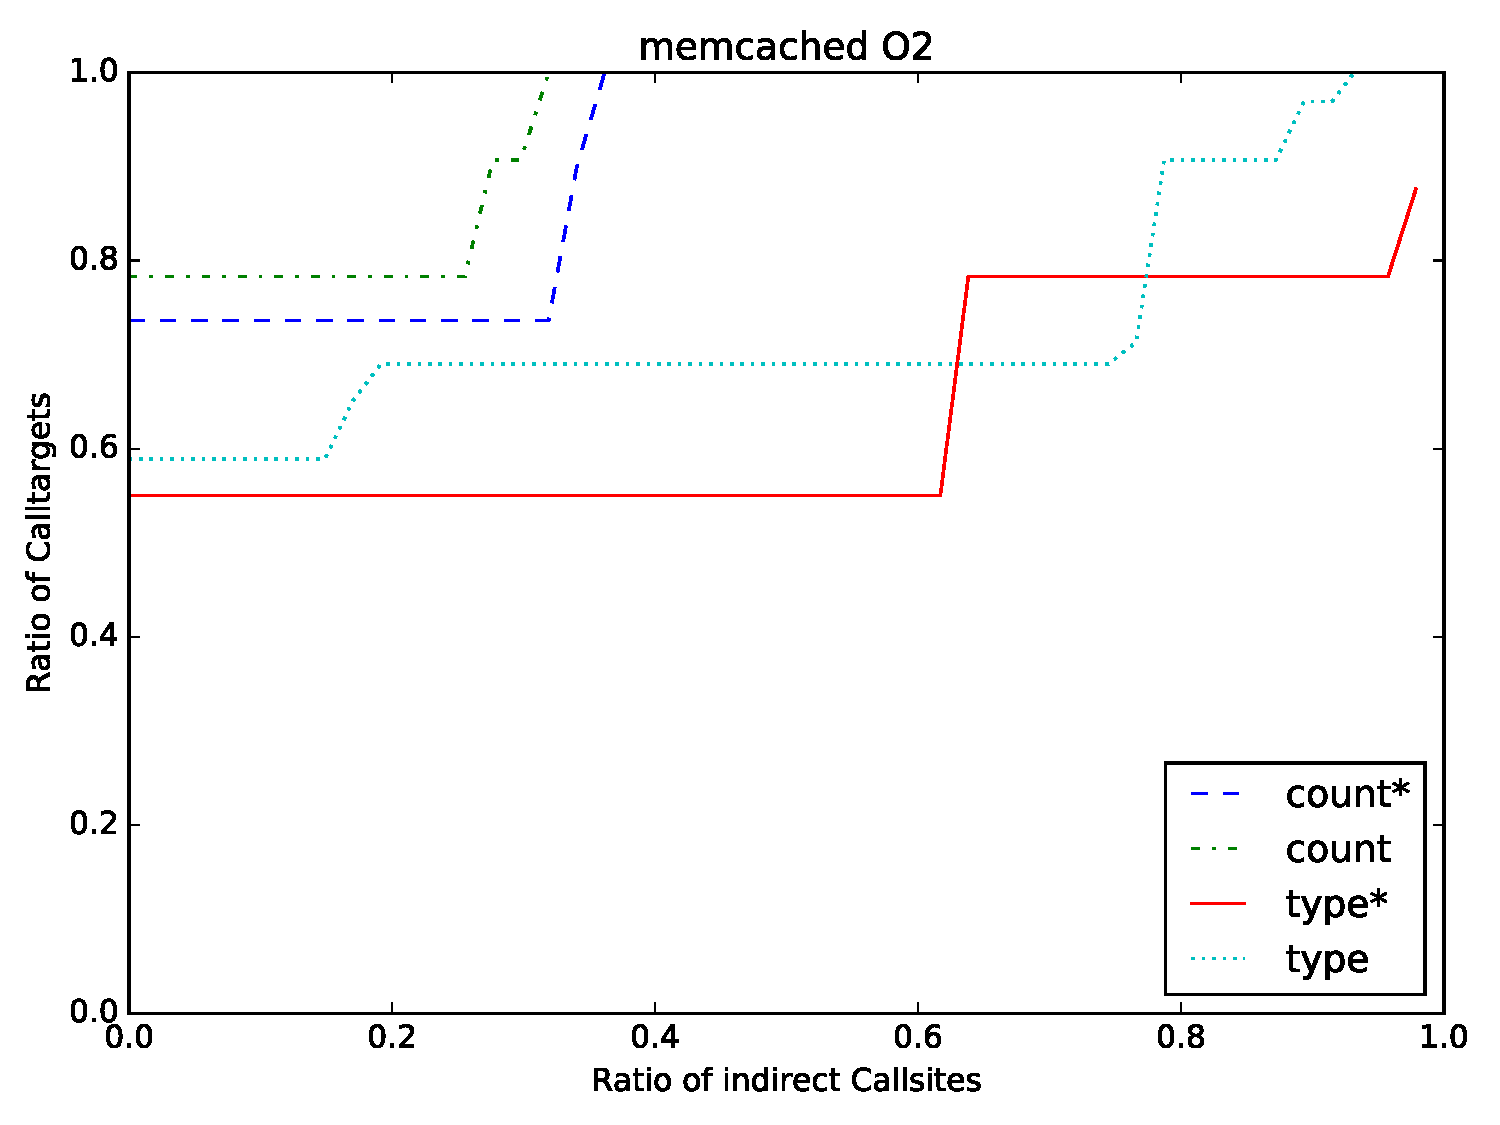
\includegraphics[width=0.5\textwidth]{../MA_Pictures/memcached.pdf}
%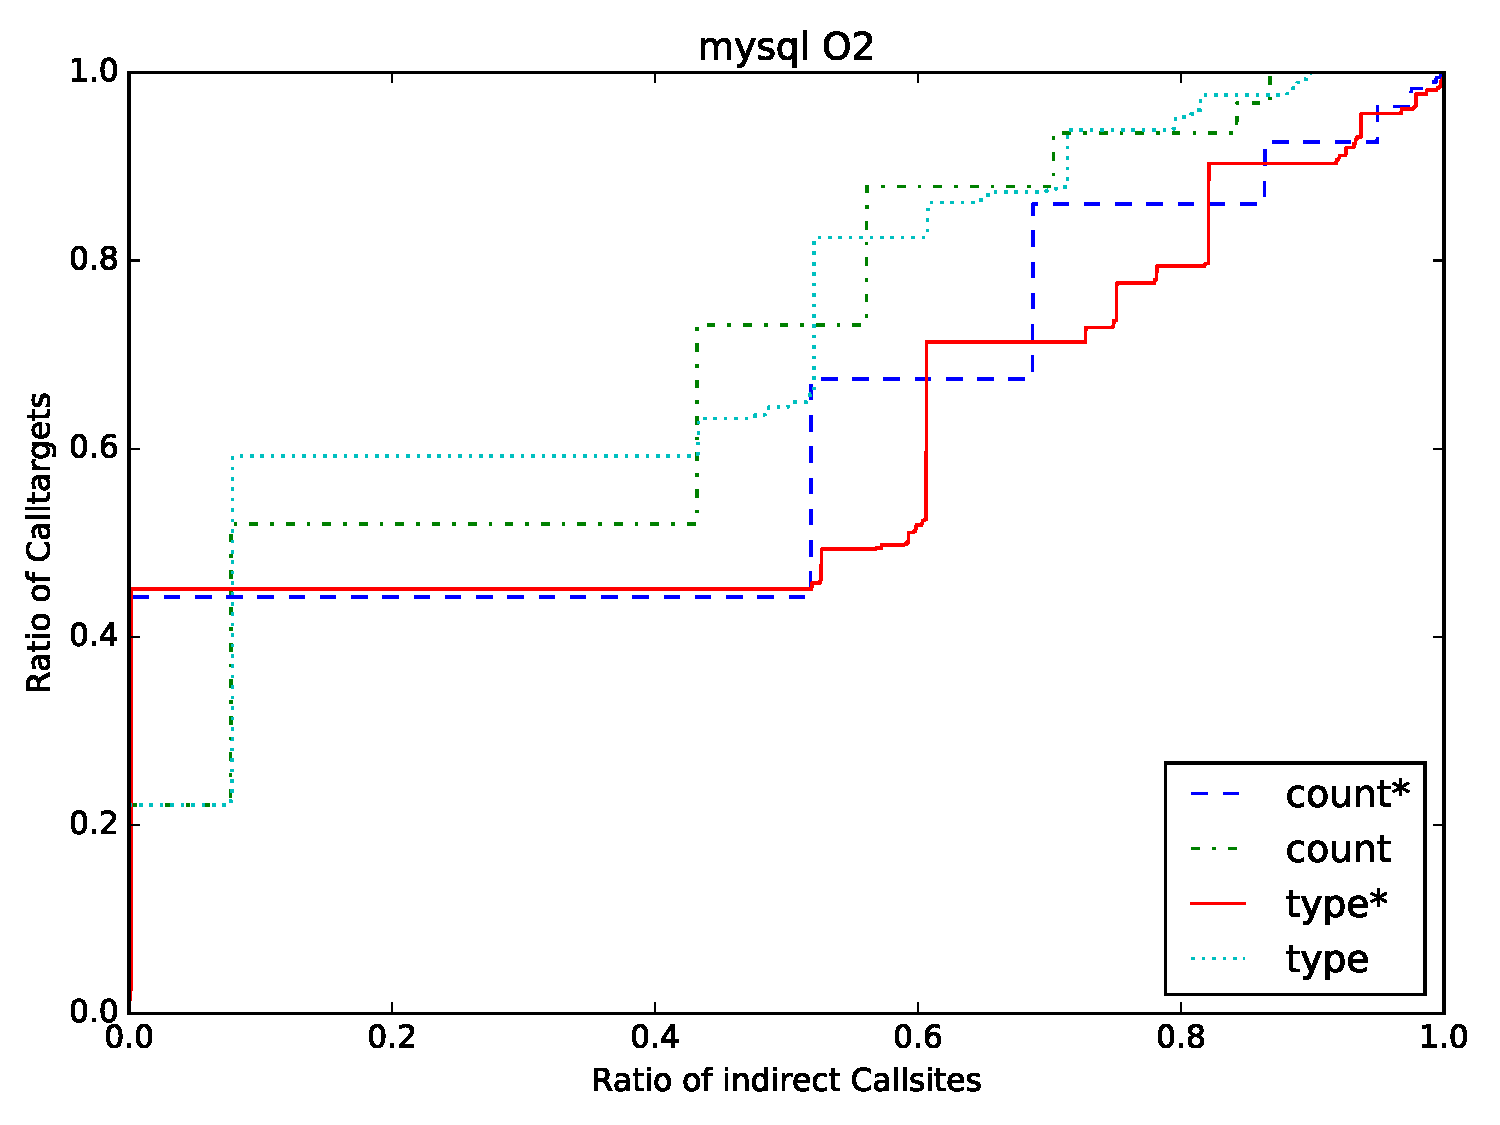
\includegraphics[width=0.5\textwidth]{../MA_Pictures/mysql.pdf}\\
%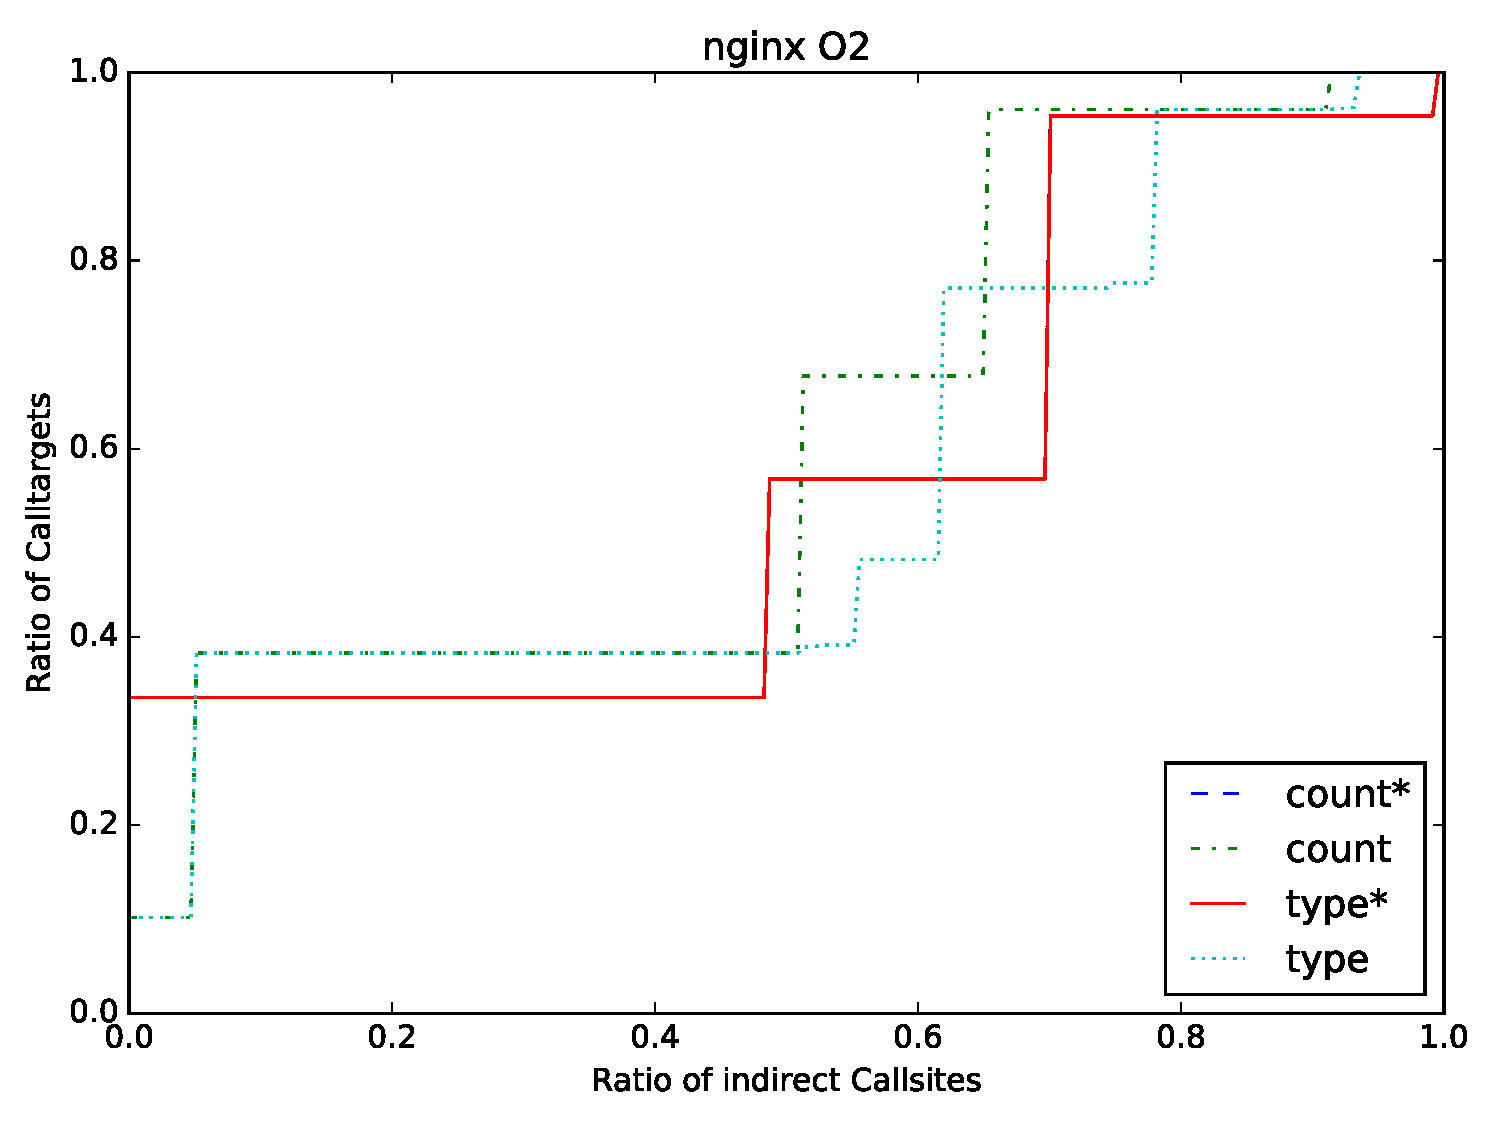
\includegraphics[width=0.5\textwidth]{../MA_Pictures/nginx.pdf}
%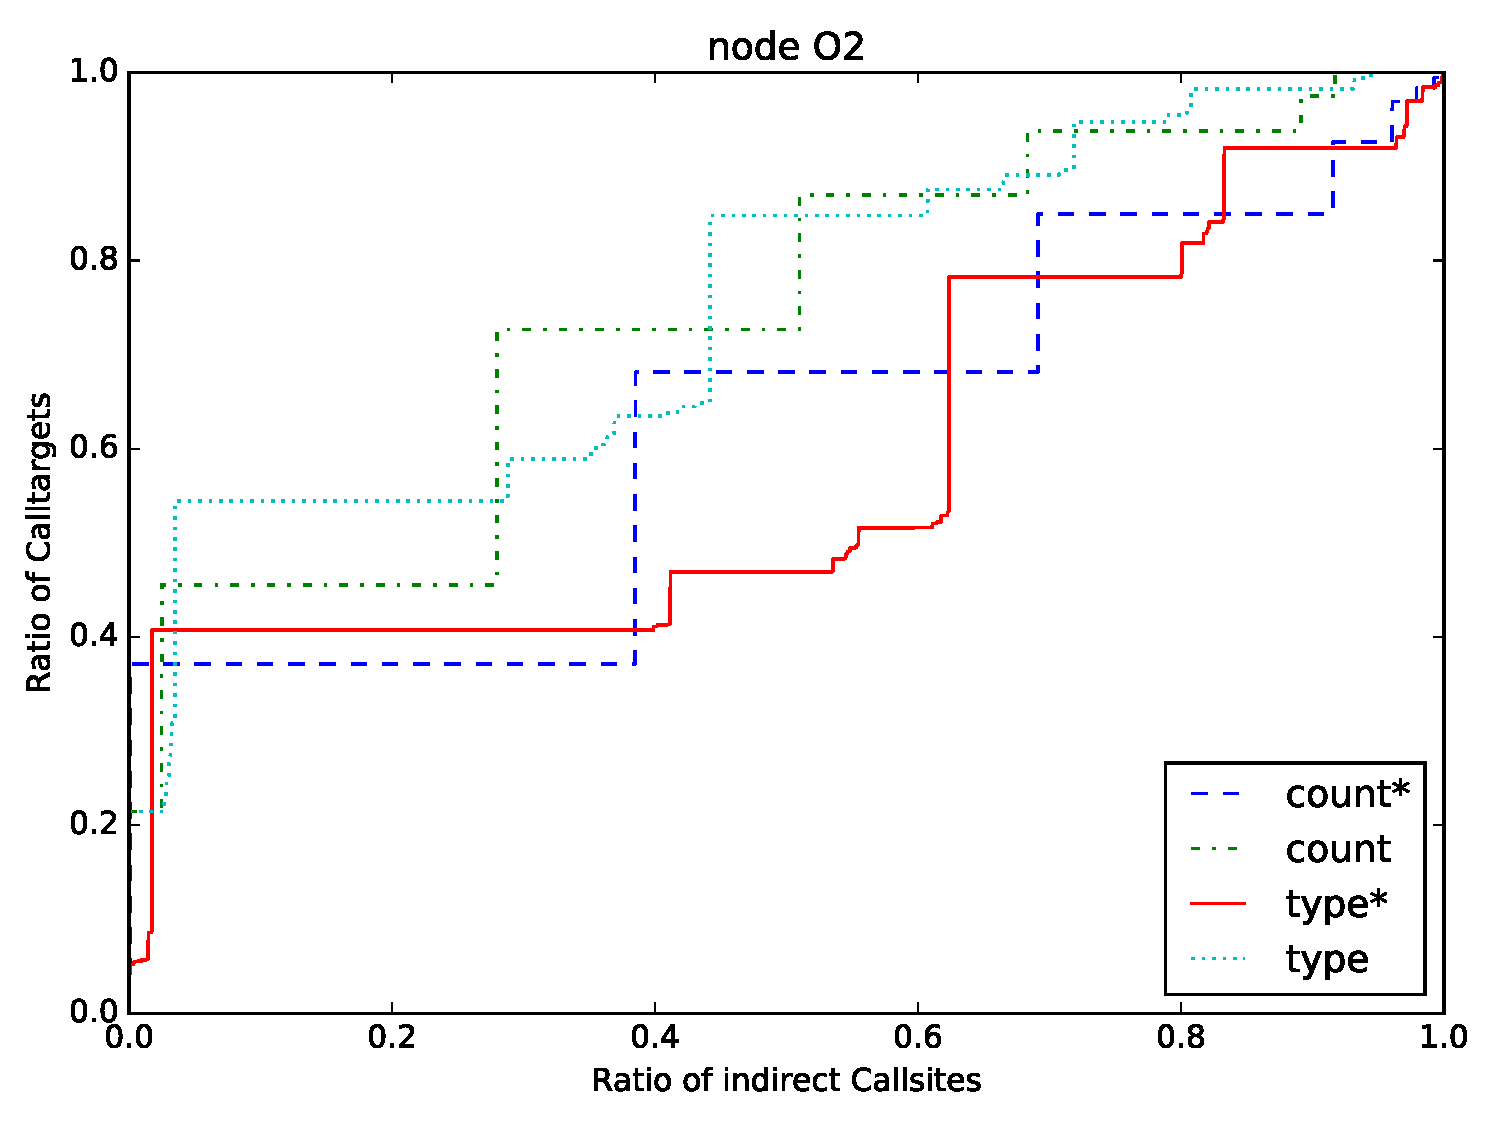
\includegraphics[width=0.5\textwidth]{../MA_Pictures/node.pdf}\\
%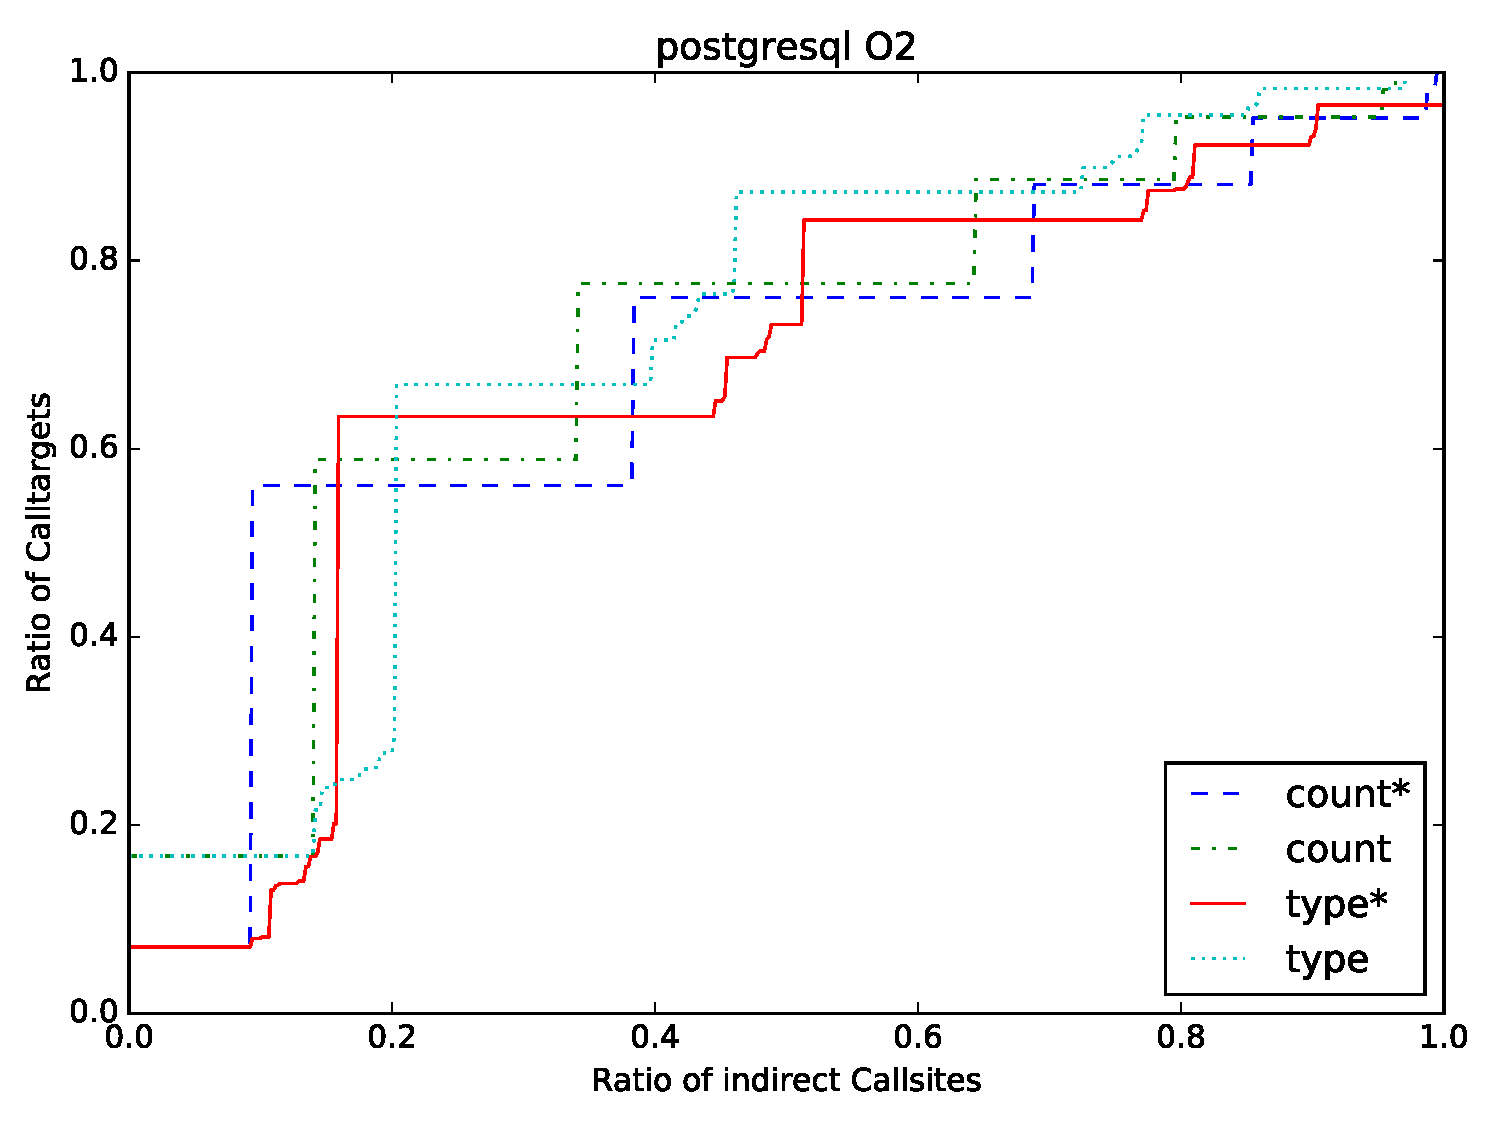
\includegraphics[width=0.5\textwidth]{../MA_Pictures/postgresql.pdf}
%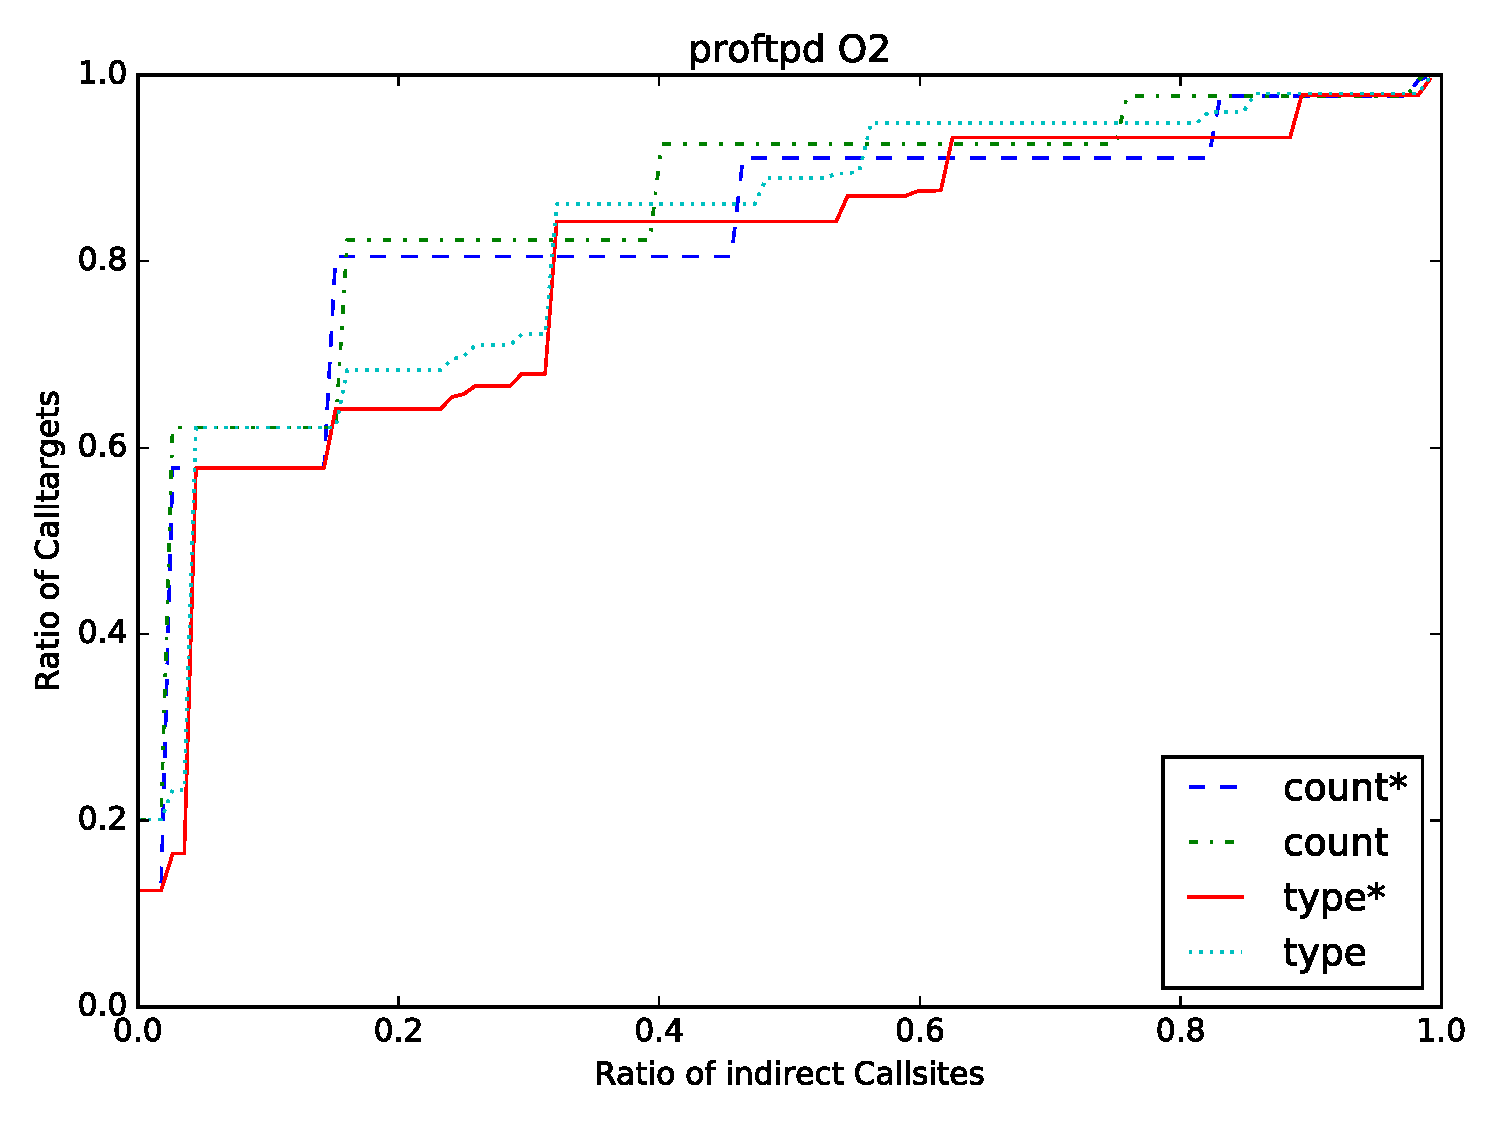
\includegraphics[width=0.5\textwidth]{../MA_Pictures/proftpd.pdf}
%\end{figure}
%

\subsubsection{CDF Analysis}
\label{CDF Analysis}

\begin{figure}[ht] 
  \label{ fig7} 
  \begin{minipage}[b]{0.5\linewidth}
    \centering
    \resizebox{1.04\columnwidth}{!}{\includesvg{postgresqlO2}}
    \caption{postgresql} 
    \vspace{4ex}
  \end{minipage}%%
  \begin{minipage}[b]{0.5\linewidth}
    \centering
    \resizebox{1.04\columnwidth}{!}{\includesvg{nodeO2}} 
    \caption{node.js} 
    \vspace{4ex}
  \end{minipage} 
  \begin{minipage}[b]{0.5\linewidth}
    \centering
    \resizebox{1.04\columnwidth}{!}{\includesvg{proftpdO2}}
    \caption{proftpd} 
    \vspace{4ex}
  \end{minipage}%% 
  \begin{minipage}[b]{0.5\linewidth}
    \centering
    \resizebox{1.04\columnwidth}{!}{\includesvg{mysqlO2}} 
    \caption{mysql} 
    \vspace{4ex}
  \end{minipage} 
\end{figure}

When looking at the CDFs of legal callsite targets as shown for postgresql \ref{fig7}, node.js \ref{fig8}, proftpd \ref{fig9}, mysql \ref{fig10}, one should instantly see the difference between the type and the count policies. While the count  policies have only a few number of changes, the number of changes that can be seen within the type policies is vastly higher. The reason for that is simple, the number of buckets that are used to classify the callsites and calltargets is simply higher. While type policies mostly perform better than the count policies, there are still parts within the type plot that are above the count plot, the reason for that is relatively simple: the maximum number of calltargets a callsite can access has been reduced, therefore a lower amount of calltargets is a higher percentage than before. However all of that is also dependent on the structure of the program.

\subsection{RQ3: Runtime Performance Overhead}
In general, we have usually about 2\%-5\% performance drop when instrumenting using Dyninst. The reason for that are essentially cachemisses introduced by jumping between the old and the new executable section of the binary generated by duplicating and patching the duplicate. This is necessary, because when out side of the compiler it is nigh on impossible to relocate indirect controlflow, therefore everytime an indirect control flow occurs, one jumps into the old executable section and from there back to the new executable section. Mroeover this is also dependent on the actual structure of the target, as it depends on the number of indirect controlflow operations per time unit.

\label{section:typeshieldoverheadperformance}
\todo[inline]{In this section we need one or two Table similar to what TypeArmor contains, first we need to define the fields which make most sense.}
\begin{figure}[htbp!]
    \centering
    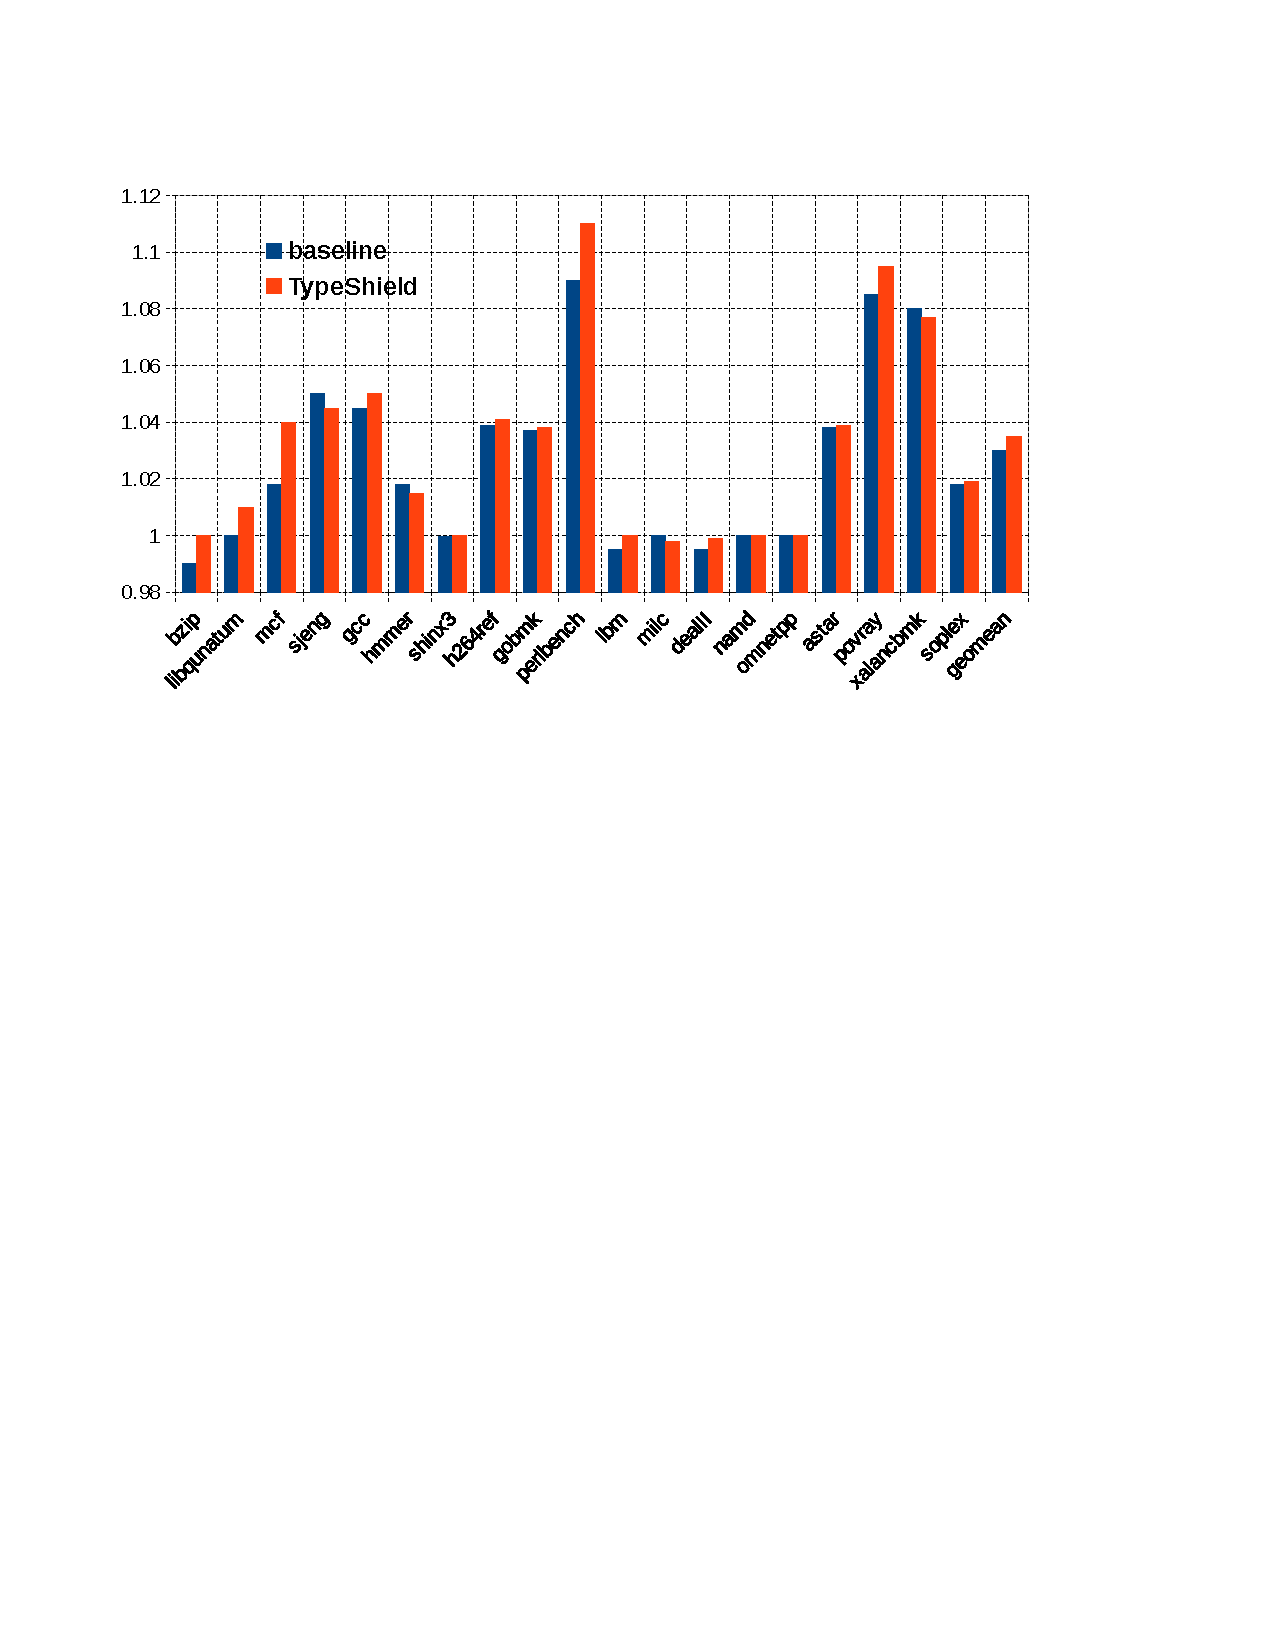
\includegraphics[width=0.49\textwidth]{figures/speccpu2006.pdf}
    \caption{Awesome Image}
    \label{fig:awesome_image}
\end{figure}
\todo[inline]{add a binary patch that does not crash none of the programs from SPEC2006.}
\todo[inline]{need a table with all the results for each of the SPEC2006 programs and a bar diagram}

\subsection{RQ4: Instrumentation Overhead}
\label{section:typeshieldoverheadinstrumentation}

\todo[inline]{here we need a bar chart, see TypeArmor paper.}
\todo[inline]{Measure the size (in bytes) of the SPEC2006 testes in RQ3 before and after adding all the patches}

The instrumentation overhead or the change in size due to patching is mostly due to the method Dyninst uses to patch binaries. 
Essentially the executable part of the binary is duplicated and extended with the patch. The usual ratio is around 40\% to 
60\% while postgres has an increase of 150\% in binary size. One cannot reduce that value significantly, 
because of the nature of code relocation after losing the data that a compiler has. Especially indirect control flow 
changes are very hard to relocate. Therefore instead each important basic block in the old code contains a jump 
instruction to the new position of the basic block.

\subsection{RQ5: Comparisons with Other Tools}
\label{RQ5: Is TypeShield better than other tools?}
\begin{table}[h!]
\resizebox{\columnwidth}{!}{
	\begin{tabular}{l|r|r|r|r|r}%
	\toprule
	\bfseries Target & AT & TypeArmor  &  IFCC &  TypeShield (count) & TypeShield (type)% specify table head
	\\\midrule
	\csvreader[before filter=\ifthenelse{\equal{\csvcolii}{geomean}}{\csvfilterreject}{\csvfilteraccept},  late after line=\\, late after last line=\\\midrule]{csvs/tools_compare.csv}{
		%1=\target, 2=\opt, 3=\fns, 4=\fnsnotClang, 5=\fnsnotpadyn, 6=\ats, 7=\atnotClang, 8=\atnotpadyn, 9=\cscount, 10=\csClang, 11=\cspadyn
	}
	{\csvcolii & \csvcoliii & \csvcoliv & \csvcolv & \csvcolvi & \csvcolvii}% specify your coloumns here

	\csvreader[before filter=\ifthenelse{\equal{\csvcolii}{geomean}}{\csvfilteraccept}{\csvfilterreject},  late after line=\\, late after last line=\\\bottomrule]{csvs/tools_compare.csv}{
		%1=\target, 2=\opt, 3=\fns, 4=\fnsnotClang, 5=\fnsnotpadyn, 6=\ats, 7=\atnotClang, 8=\atnotpadyn, 9=\cscount, 10=\csClang, 11=\cspadyn
	}
	{\csvcolii & \csvcoliii & \csvcoliv & \csvcolv & \csvcolvi & \csvcolvii}% specify your coloumns here
    	\end{tabular}}
%     	}
	\caption {The medians of calltargets per callsite for different tools that we have values for}
	\label{tbl:toolcompare}
\end{table}

Table~\ref{tbl:toolcompare} depicts a comparison between \textsc{TypeShield}, TypeArmor and IFCC w.r.t. the count of calltargets per callsites.
The values depicted in this table for TypeArmor and IFCC are taken from the original TypeArmor paper.
We compare our version of address taken analysis (AT), TypeArmor, TypeShield (count), TypeShield (type) and IFCC. 
The first thing to notice is that when comparing these values, one can see that we did not implemented a separation based on return type or the 
CFC that TypeArmour introduced. Therefore when implementing those measures, we predict that our solution would improve even more in w.r.t precision.
While we think it is possible to surpass TypeArmor implementing those two solutions in our tool, we deem it nigh on impossible to be able to compete with IFCC,
which can directly operate on the sourcecode level. Therefore it has access to more possibilities than simply inspecting the parameters or return values.






% \section{Discussion}
\label{chapter:Discussion}

\textbf{Comparison with TypeArmor.}
\label{section:comptype}
We are looking at two sets of results. First of all, we compare the overall precision of our implementation
of the COUNT policy with the results from TypeArmor to set the perspective for the precision of our TYPE 
policy. We cannot compare data regarding overestimations of calltargets or underestimations of callsites, 
as TypeArmor did not provide sufficient data. The second point of comparison is the reduction of calltargets
per callsite, however, this comparison is rather crude, as we most surely do not have the same measuring
environment and not sufficient data to infer its quality.

\textit{Precision of Classification.}
TypeArmor reports a geometric mean of 83.26\% for the perfect classification of calltargets regarding 
parameter count in optimization level O2, which compares rather well to our result of 82.24\%. Regarding
the perfect classification of callsites we report a geometric mean of 81.6\% perfect classification 
regarding parameter count, while TypeArmor reprots a geometric mean of 79.19\%. Howevver we also have
a geometric mean of about 7\% regarding underestimations in the callsite classification with an upper
bound of 16\%, while TypeArmor reports that it does not incur underestimations in their callsites.
Now, for our type based classification we incur the cost for two error sources. First, the error from
the parameter count classification, which we base our type analysis on and second for the type analysis
itself. The numbers for the perfect classification of calltargets regarding parameter types we report a
72.25\% geometric mean of perfect classification, which is 87.85\% of our precision regarding parameter
counts. However we report a geometric mean of 57.36\%
for perfect classification of callsites, which altough seemingly low, is still 69.74\% of our precsion
regarding parameter counts.

\textit{Reduction of Available Calltargets}
While our count based precision focused implementation achieves a reduction in the same ballpark as
TypeArmour regarding our test targets, lets us believe that our implementation of their classification
schema is a sufficient approximation to compare against. However, we cannot safely compare those numbers,
as the information regarding their test environment are rather sparse and the only data available is the
median, which in our opinion does discard valuable information from the actual result set. This is the
main reason we implemented an approximation, because we needed more metrics to compare \textsc{TypeShield}
and TypeArmor regarding calltargets. Using average and sigma, we can report that our precision focused
type based classification can reduce the number of calltargets, by up to 20\% more than parameter number
based classification with an overall reduction of about 9\%.


\textbf{TypeArmor Discrepancies.}
\label{section:discrep}
As we have no access to source code of TypeArmor, we habe implemented an approximation
of TypeArmor. Using this approximation we found some discrepancies between the data that we collected
and data that was presented.
A minor discrepancy between our results and the results of TypeArmor is that, while they basically implemented
what we call a destructive merge operator for the liveness analysis. However, our data suggestes that this
operator is marginally inferior to the union pathmerge operator, when we compared them in our implementation.
A major concern is the classification of calltargets, while we were able to reduce the number of overerstimations
of calltargets regarding parameter counts to essentially 0, the number of underestimations of calltarget did
stay at a geometric mean of 7\%. This error rate is rather large when compared to the reported 0\% underestimation
of TypeArmor, however we are not entirely sure what has caused this discrepancy. A possibility is the differing
test environments, or a bug within our implementation that we are not aware of, or simply reaching defintions
analysis alone is not the best possible algorithm for this particular problem.

\textbf{Improving \textsc{TypeShield}.}
\label{section:venuesimp}
To improve our type analysis, we see atleast two possibilities. Incorporating refined dataflow analysis and 
expanding the scope to also include memory. The main point of improvement is not the precision but for now 
more importantly the reduction of underestimations in the callsite analysis.

To refine the dataflow analysis, we propse the actual tracking of data values and simple operations, as these
can be used to better differentiate the actual wideness stored within the current register. The highest gain, 
we see here would be the establishment of upper and lower bounds regarding values within the register, which 
would allow for more sophisticated callsite and calltarget invariants. Essentially we would have to resort 
to symbolic execution or some other sort of precise abstract interpretation.

Expanding the scope to also include memory, is another possible way of improving the type analysis, as it 
would allow us to distinguish normal 32 or 64 bit values and pointer addresses. Although we already have a 
limited approach of that in our reaching implementation, we still see room for improvement, as we only check
whether a value is within one of three binary sections or 0.

\textbf{Limitations of \textsc{TypeShield}.}
\label{section:limit}
First of all, we are limited by the capabilities of the DynInst Instrumentation Environment, the main problem,
we are facing here is that non returning functions like exit are not detected reliably in some cases, which is
why we were not able to test the Pure-FTP server, as it heavily relies on these functions. The problem is that
those non returning functions usually appear as a second branch within a function that occurs after the normal
control flow, causing basic blocks from the following function to be attributed to the current function. This
results in a malformed control flow graph and erroneous attribution of callsites and problematic misclassifications
for both calltargets and callsites.

Another limitation of \textsc{TypeShield} is it reliance on variety within the binary, in particular we rely on
the fact that functions use more than only 64bit values or pointers within their parameter list. Should this
scenario occur, our analysis has nothing to work with and essentially degrades into a parameter count based
implementation. Thankfully this occurrence is quite rare, as we experienced within our experiments. When working
based on source level information, we could not detect a difference between our TYPE and a COUNT policies. 
However when leveraging our tool, we were able to detect differences, which reinforces the fact, that we do 
not rely on declaration of parameters but usage of those.

\section{Related Work}
\label{chapter:Related_Work}

\textbf{Type-Inference on Executables.}
\label{Type-Inference on Executables}
Recovering variable types from executable programs
is very hard in general for several reasons. 
First, the quality of the disasembly can very much from used
framework to another. \textsc{TypeShield} is based on DynInst 
and the quality of the execuatble disasembly fits our needs. 
For a more comprehensive review on the capabilities of DynInst and other tools we
advice the reader to have a look at~\cite{andriesse:indepth}.
Second, alias analysis in binares is undecidable in theory and intractable in practice~\cite{alan:mycroft}.
There are several most promising tools such as: Rewards~\cite{lin:rewards}, BAP~\cite{bap:brumley}, 
SmartDec~\cite{fokin:smartdec}, and Divine~\cite{divine:balakrishnan}.
These tools try with more or less success to recover 
type information from binary programs with different goals.
Typical goals are: 
\textit{i)} full program reconstruction (binary to code convertion, reversing), 
\textit{ii)} checking for buffer overflows, 
\textit{iii)} integer overflows and other types of memory corruptions.
For a more exhaustive review of such tools we advice the reader to
have a look at the review of Caballero et al.~\cite{caballero:inference}.
Intresting to notice is that the code from only a few of this tools is available.

While smartde seemed promising due to its simple type lattice that we wanted to leverage for our classification schema. Its integration into our DynInst based environment was not successful mostly for time constraints, as it was deemed to time consuming to extract the whole machinery and implemnt an interface to the DynInst disassembler.
Therefore we finally implemented our own version of type analysis and only focused on the wideness of the types, resulting in a simpler lattice than we initially wanted.

%maybe not relevant
\textbf{Mitigation of Code-Reuse Attacks.}
\label{Mitigation of Code-Reuse Attacks}
In the last couple of years researchers have provided many versions of new Code Reuse Attacks (CRAs).
These new attacks were possible since DEP~\cite{dep} and ASLR~\cite{ASLR} were successfully bypassed mostly based
on Return Oriented Programming (ROP)~\cite{ROP, kornau:rop, rop:shacham} on one hand and on 
the other hand due to the discovery of new exploitable hardware and software primitives.

ROP started to present itself in the last couple of years in many faceted ways such as:
Jump Oriented Programming (JOP)~\cite{JOP1, JOP2, JOP3} which uses jumps in order to divert the control flow to the next gadget and 
Call Oriented Programming (COP)~\cite{rop:carlini} which uses calls in order to chain gadgets together.
CRAs have many manifestations and it is out of scope of this work to list them all.

On one hand, CRAs can be mitigated in general in the following ways: 
\textit{(i)} binary instrumentation,
\textit{(ii)} source code recompilation and 
\textit{(iii)} runtime application monitoring.
On the other hand, there is a plethora of tools and techniques which try to enforce CFI based
primitives in executables, source code and during runtime. Next we briefly
present the solution landscape together with the approaches and the techniques on which these are based:
\textit{(a)} fine-grained CFI with hardware support, PathArmor~\cite{veen:cfi},
\textit((b)) coarse-grained CFI used for binary instrumentation, CCFIR~\cite{ccfir:zhang},
\textit{(c)} coarse-grained CFI based on binary loader, CFCI~\cite{cfci:zhang}
\textit{(d)} fine-grained code randomization, O-CFI~\cite{mohan:opaque},
\textit{(e)} cryptografy with hardware support, CCFI~\cite{ccfi:jose},
\textit{(f)} ROP stack pivoting, PBlocker~\cite{pblocker:prakash},
\textit{(g)} canary based protection, DynaGuard~\cite{dynaguard:petsios},
\textit{(h)} runtime and hardware support based on a combination of LBR, PMU and BTS registers CFIGuard~\cite{cfiguard:yuan}, and
\textit{(i)} source code recompilation with CFI and/or randomization enforcement against JIT-ROP attacks, MCFI~\cite{mcfi:niu}, 
RockJIT~\cite{rockjit:niu} and PiCFI~\cite{perinput:niu}.

The above list is not exhaustive and new protection techniques can be obtained by combining available techniques
or by using newly available hardware features or software exploits. However, none of the above techniques and tools 
can mitigate against COOP attacks.


% \textbf{Mitigation of Advanced Code-Reuse Attacks.}
\textbf{Mitigation of Forward-Edge based Attacks.}
\label{Mitigation of Advanced Code-Reuse Attacks}
Recur-sive-COOP~\cite{crane:readactor++}, COOP~\cite{schuster:coop} and Subversive-C~\cite{subversive-c:lettner}.
are advanced CRAs since these attacks can not be addressed:
\textit{i)}  with shadow stacks techniques (i.e., do not violate the caller/calle convention), 
\textit{ii)} coarse-grained Control-Flow Integrity (CFI)~\cite{abadi:cfi2, abadi:cfi} techniques are useless against these attacks, 
\textit{iii)} hardware based approaches such as Intel CET~\cite{intel:cet} can not mitigate this attack for the same reason as in \textit{i)}, and 
\textit{iv)} with OS-based approaches such as Windows Control Flow Guard~\cite{windows:cfguard} 
since the precomputed CFG does not contain edges for indirect call sites which are explicitly exploited during the COOP attack.
However, the following tools can protect against COOP attacks:

\textit{Source code based.} Indirect call site targets are checked based on vTable integrity.
Different types of CFI policies are used such as in the following tools:
SafeDispatch~\cite{safedispatch:jang}, IFCC/VTV~\cite{vtv:tice} LLVM and GCC compiler.
Additionally, the Redactor++~\cite{crane:readactor++} uses randomization 
vTrust~\cite{zhang:vtrust} checks call target function signatures, 
CPI~\cite{volodymyr:cpi} uses a memory safety technique
in order to protect against the COOP attack.

There are several source code based tools 
which can successfully protect against the COOP attack.
Such tools are: ShrinkWrap~\cite{haller:shrinkwrap}, IFCC/VTV~\cite{vtv:tice}, 
SafeDispatch~\cite{safedispatch:jang}, vTrust~\cite{zhang:vtrust}, Readactor++~\cite{crane:readactor++}, CPI~\cite{volodymyr:cpi} and the
tool presented by Bounov et al.~\cite{bounov:interleaving}. These tools profit from high precision
since they have access to the full semantic context of the program though the scope
of the compiler on which they are based. 
Because of this reason these tools target mostly other types of security problems than binary-based 
tools address. For example some last advancec in compile based protection against 
code reuse attacks address mainly performance issues.
Currently, most of the above presented tools are only forward
edge enforcers of fine-grained CFI policies with an overhead from 1\% up to 15\%.

We are aware that there is still a long research path to go until binary based techniques can 
recuperate program based semantic information from executable with the same precision as compiler based tools.
These path could be even endless since compilers are optimized for speed and are designed to remove as much as possbile semantic information
from an executable in order to make the program run as fast as possible. In light of this fact,
\textsc{TypeShield} is another attempt to recuperate just the needed semantic information (types and number of function parameters from
indirect call sites) in order to be able to enforce a precise and with low overhead primitive against COOP attacks.

Rather than claiming that the invariants offered by \textsc{TypeShield} are suffiecient
to mitigate all versions of the COOP attack we take a more conservative path by claiming that \textsc{TypeShield} 
further raises the bar w.r.t. what is possible when defending against COOP attacks on the binary level.

\textit{Binary based.} vTable protection is addressed through binary instrumentation in tools
such as: vfGuard~\cite{vfuard:aravind}, vTint~\cite{vtint:zhang}. However, none of these tools can
help to mitigate against COOP. The only binary based tool which we are aware of that
can mitigate protect against COOP is TypeArmor~\cite{veen:typearmor}.  
TypeArmor uses a fine-grained CFI policy based on caller (only indirect call sites)/callee matching 
which consists in checking during runtime if the number of provided and needed parameters match.

\textsc{TypeShield} is most similar to TypeArmor~\cite{veen:typearmor} since
we also enforce strong binary-level invariants on the number of function
paramters. \textsc{TypeShield} similarly to TypeArmor targets 
exclusive protection against advanced exploitation techniques 
which can bypass fine-grained CFI schemes and VTable protections at the binary level.

However, \textsc{TypeShield} offers a better restriction of call targets to call sites, since 
we not only restrict based on the number of parameters but also on the wideness of their types. 
This results in much smaller buckets that in turn can only target a smaller subset of all address
taken functions. However, we rely for that on the variety of parameter types and when there is 
none, we will degrade into a parameter count policy.

\textit{Runtime based.}
``There is something available out there but I can not use it'' \textit{Anonymous}.
Long story short conclusion: There are several promising runtime-based line of defenses against
advanced CRAs but none of them can successfully protect against the COOP attack.

IntelCET~\cite{intel:cet} is based on, \texttt{ENDBRANCH}, a new CPU instruction which can be used to enforce
an efficient shadow stack mechanism. The shadow stack can be used to check during program execution if caller/return pairs match.
Since the COOP attack reuses whole functions as gadgets and does not violate the caller/return convention than the 
new feature provided by intel is useless in the face of this attack. Nevertheless other highly notorious CRAs may not be possible
after this feature will be implemented main stream in OSs and compilers.

Windows Control Flow Guard~\cite{windows:cfguard} is based on a user-space and kernel-space components which
by working closely together can enforce an efficient fine-grained CFI policy based on a precomputed CFG.
These new feature available in Windows 10 can considerably rise the bar for future attacks but in our opinion advanced CRAs
such as COOP are still possible due the typical characteristics of COOP.

PathArmor~\cite{veen:cfi} is yet another tool which is based on a precomputed CFG and on the LBR register which can give a string of 16 up to
32 pairs of from/to addressed of different types of indirect instructions such as \texttt{call}, \texttt{ret}, and \texttt{jump}. 
Because of the sporadic query of the LBR register (only during invocation of certain function calls) and because of the sheer amount of 
data which passes through the LBR register this approach has in our opinion a fair potential to catch different types of CRAs but
we think that against COOP this tool can not be used. First, because of the fact that the precomputed CFG does not contain edges for all
possible indirect call sites which are accessed during runtime and second, the LBR buffer can be easily triked by adding
legitimate indirect call sites  during the COOP attack.


% \section{Future Work}
\label{chapter:Future_Work}
\textbf{Structural matching capability.} 
Improving the structural matching capability is in our opinion the most 
important further venue of research, as we need a reliable way to 
match a ground truth against the resulting binary. This is important 
because it is a prerequisite to the ability to generate reliable 
measurements and reduces the current uncertainty (\textit{i.e.,} we rely on the 
number of calltargets per callsite to match callsites and furthermore
assume that the order within ground truth and binary is the same).

\textbf{Better patching schema.} 
Devising a patching schema
that is based on Dyninst functionality, 
which allows annotation of calltargets so they can hold at least 
4-byte of arbitrary data. This is required to hold the type data that
we generate using our classification. Keeping the runtime overhead
of said patching schema low should be the second goal of this venue 
after satisfying stability.

\textbf{Expanding to return values.} 
Expanding our schema to return values
is another viable venue of further work, as we were not able to 
reliably reduce the number of problematic classification regarding 
the return values of functions to 
manageable levels. Should one attempt this, it should be noted that the
responsibilities of callsites and calltargets are reversed in this 
case: The callsite requires return value wideness, while the calltarget
needs to provide it.

\textbf{Using pointer/memory analysis.} 
Introducing pointer/memory analysis
to distinguish simple 32-bit and 64-bit values and actual addresses to even further restrict the 
possible number of calltargets per callsite. This would require more 
precise data flow analysis, as in calculating value possibilities for 
registers at each instruction.

\section{Conclusion}
\label{chapter:Conclusion}
%version 1
% In this paper, we introduced \textsc{TypeShield} a tool for binary harding of forward indirect
% calls based on function parameter type and count.
% Advanced code reuse attacks such as COOP and its extensions or Control Jujutsu manifest due to a combination of facts and problems, 
% like memory corruption or predictable binary layout and the fact that the larger our binaries get, the 
% higher the chance they contain useful gadgets for an attacker. However, due to their nature, traditional 
% CFI cannot detect them, as they do not actually replace code to modify the control flow, but change pointers
% in memory, which redirects the targets of indirect callsites, which are uncertain at the time of compilation. 
% Two of the most common targets are the pointers to virtual function tables to implemented inheritance in C++ 
% and global function pointers. The control flow exhibited by the binary while functioning normal and while 
% under attack will seem the same. Address taken analysis alread helped cutting down the number of possible 
% calltargets one could inject by a considerable amount. And typearmor improved on that by implementing 
% invariants for both callsites and calltargets based on the number of parameters. We had no access to
% their sourcecode and therefore had to rely on their paper to implement an approximation for which 
% we generated comparable results regarding precision. We improved on that solution by implementing \textsc{TypeShield}, 
% which allows for a more fine-grained classification of calltargets and indirect callsites by implementing a rather 
% simplistic register wideness based type analysis. However, as simplistic as that analysis might be, we showed that 
% except for special cases (nginx), we were able to improve upon a parameter count based implementation by reducing 
% the average target count by about 20\%.



%version 2
% The family of forward indirect call based attacks which can manifest due to a series of factors such as
% memory corruptions, binary layout leackages and availability of useful
% gadgets in a sufficiently large executable poses a serious security threat.
In this paper, we presented \textsc{TypeShield}, a runtime fine-grained CFI-enforcing tool which 
operates on program binaries. Our tool precisely and efficiently filters legitimate from 
illegitimate forward indirect control flow transfers by using a novel runtime type-checking 
technique based on function parameter type-checking and parameter-counting. 
%Further, we maintain a comparable performance overhead to existing tools. (REDUNDANT WITH BELOW)

We have implemented~\textsc{TypeShield} and applied it to real software such as web servers, FTP servers and the SPEC CPU2006 benchmark. 
We demonstrated through extensive experiments that~\textsc{TypeShield} has 
higher precision than existing state-of-the-art tools, while maintaining a comparable runtime performance overhead. 
To date, we were able to improve on parameter count based techniques by reducing the possible calltargets per 
callsite ratio by 20\% with an overall reduction of about 9\% when comparing with similar state-of-the-art approaches. 
Next to a more precise analysis, the tangible outcome is a considerably reduced attack surface.
In the spirit of open research, we have made the source code of \textsc{TypeShield} and the evaluation results publicly available 
at \url{https://github.com/stub/typeshield}, thus we support reproducibility in this fast-moving 
research field by providing comprehensive descriptions of our experiments.




%todos list
% \listoftodos

%the bibliography

\bibliographystyle{IEEEtran} 
% \bibliographystyle{sigplanconf-eurosys} 
\bibliography{literatur}  



% \theendnotes

%appendix, taken out for now.
% \section*{Appendix}
\label{appendix}

\begin{figure}[h!]
\centering
\resizebox{0.25\textwidth}{!}{
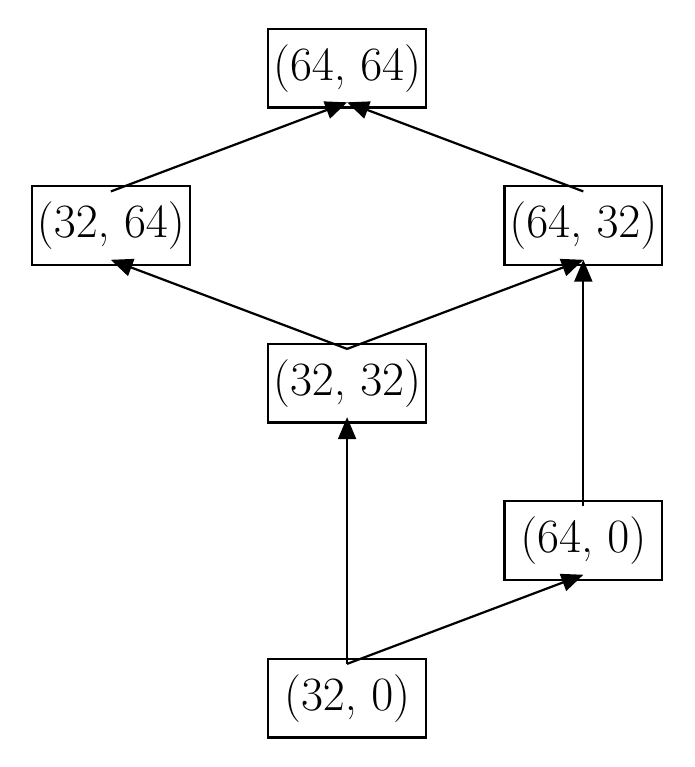
\begin{tikzpicture}

\draw[thick] (0,0) rectangle node[anchor=center]  (320)  {\LARGE{(32, 0)}}  (2,-1);

\draw[thick] (3,2) rectangle node[anchor=center]  (640)  {\LARGE{(64, 0)}}  (5,1);

\draw[thick] (0,3) rectangle node[anchor=center]  (3232) {\LARGE{(32, 32)}} (2,4);

\draw[thick] (3,5) rectangle node[anchor=center]  (6432) {\LARGE{(64, 32)}} (5,6);
\draw[thick] (-1,5) rectangle node[anchor=center] (3264) {\LARGE{(32, 64)}} (-3,6);

\draw[thick] (0,7) rectangle node[anchor=center]  (6464) {\LARGE{(64, 64)}} (2,8);

  \draw[draw, -triangle 45, thick] (3264.north) -- (6464.south);
  \draw[draw, -triangle 45, thick] (6432.north) -- (6464.south);
  \draw[draw, -triangle 45, thick] (3232.north) -- (3264.south);
  \draw[draw, -triangle 45, thick] (3232.north) -- (6432.south);
  
  \draw[draw, -triangle 45, thick] (640.north) -- (6432.south);
  \draw[draw, -triangle 45, thick] (320.north) -- (3232.south);
  \draw[draw, -triangle 45, thick] (320.north) -- (640.south);
  
\end{tikzpicture}
}
\caption{Example for the wideness based schema when only using a parameter wideness of 64, 32 and 0 bits and only two parameters.}
\label{fig:lattice3264}
\end{figure}


\begin{figure}[!h]
\center
\hspace*{-.2cm} 
\resizebox{0.5\textwidth}{!}{
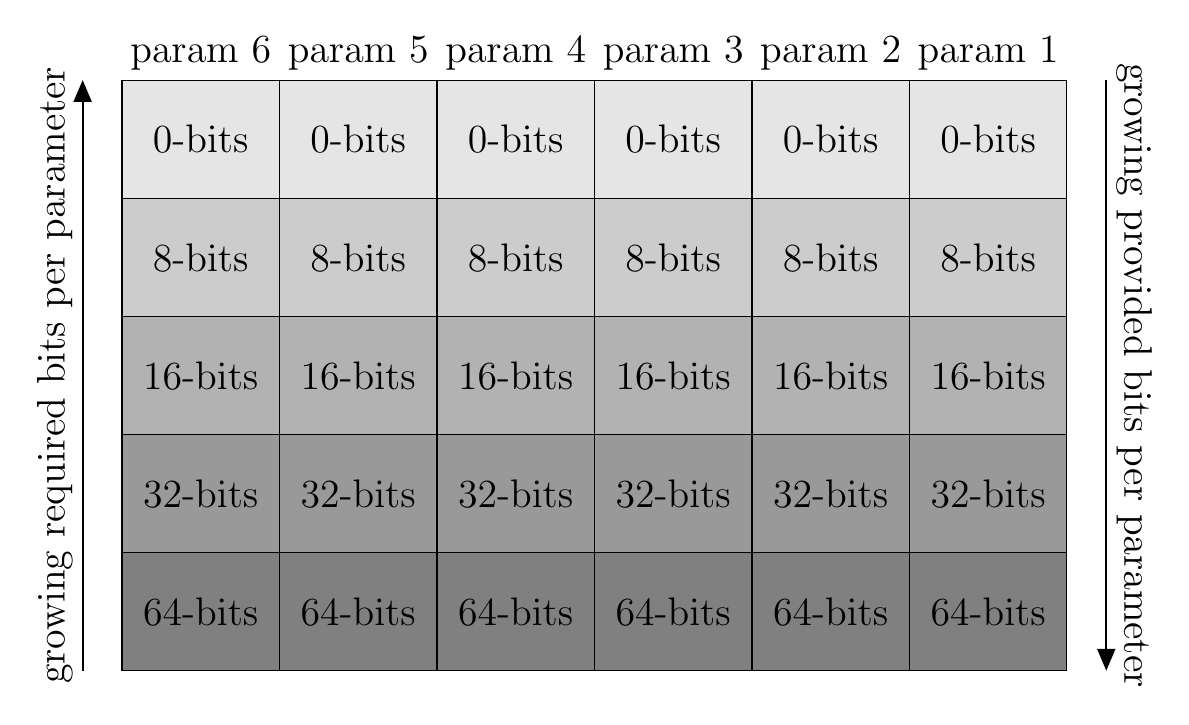
\begin{tikzpicture}

\fill[black!10!white] (0,7.5) rectangle (12,6);
\fill[black!20!white] (0,6) rectangle (12,4.5);
\fill[black!30!white] (0,4.5) rectangle (12,3);
\fill[black!40!white] (0,3) rectangle (12,1.5);
\fill[black!50!white] (0,1.5) rectangle (12,0);

\draw[-triangle 45, thick] (-0.5,0) -- node[sloped, anchor=center, above] {\Large{growing required bits per parameter}} (-0.5,7.5);
\draw[-triangle 45, thick] (12.5,7.5) -- node[sloped, anchor=center, above] {\Large{growing provided bits per parameter}} (12.5,0);

\draw (0,7.5)  --node[anchor=south] {\Large{param 6}} (2,7.5);
\draw (2,7.5)  --node[anchor=south] {\Large{param 5}} (4,7.5);
\draw (4,7.5)  --node[anchor=south] {\Large{param 4}} (6,7.5);
\draw (6,7.5)  --node[anchor=south] {\Large{param 3}} (8,7.5);
\draw (8,7.5)  --node[anchor=south] {\Large{param 2}} (10,7.5);
\draw (10,7.5) --node[anchor=south] {\Large{param 1}} (12,7.5);

\draw (0,7.5)  rectangle node[anchor=center] {\Large{0-bits}} (2,6);
\draw (2,7.5)  rectangle node[anchor=center] {\Large{0-bits}} (4,6);
\draw (4,7.5)  rectangle node[anchor=center] {\Large{0-bits}} (6,6);
\draw (6,7.5)  rectangle node[anchor=center] {\Large{0-bits}} (8,6);
\draw (8,7.5)  rectangle node[anchor=center] {\Large{0-bits}} (10,6);
\draw (10,7.5) rectangle node[anchor=center] {\Large{0-bits}} (12,6);

\draw (0,6)  rectangle node[anchor=center] {\Large{8-bits}} (2,4.5);
\draw (2,6)  rectangle node[anchor=center] {\Large{8-bits}} (4,4.5);
\draw (4,6)  rectangle node[anchor=center] {\Large{8-bits}} (6,4.5);
\draw (6,6)  rectangle node[anchor=center] {\Large{8-bits}} (8,4.5);
\draw (8,6)  rectangle node[anchor=center] {\Large{8-bits}} (10,4.5);
\draw (10,6) rectangle node[anchor=center] {\Large{8-bits}} (12,4.5);

\draw (0,4.5)  rectangle node[anchor=center] {\Large{16-bits}} (2,3);
\draw (2,4.5)  rectangle node[anchor=center] {\Large{16-bits}} (4,3);
\draw (4,4.5)  rectangle node[anchor=center] {\Large{16-bits}} (6,3);
\draw (6,4.5)  rectangle node[anchor=center] {\Large{16-bits}} (8,3);
\draw (8,4.5)  rectangle node[anchor=center] {\Large{16-bits}} (10,3);
\draw (10,4.5) rectangle node[anchor=center] {\Large{16-bits}} (12,3);

\draw (0,3)  rectangle node[anchor=center] {\Large{32-bits}} (2,1.5);
\draw (2,3)  rectangle node[anchor=center] {\Large{32-bits}} (4,1.5);
\draw (4,3)  rectangle node[anchor=center] {\Large{32-bits}} (6,1.5);
\draw (6,3)  rectangle node[anchor=center] {\Large{32-bits}} (8,1.5);
\draw (8,3)  rectangle node[anchor=center] {\Large{32-bits}} (10,1.5);
\draw (10,3) rectangle node[anchor=center] {\Large{32-bits}} (12,1.5);

\draw (0,1.5)  rectangle node[anchor=center] {\Large{64-bits}} (2,0);
\draw (2,1.5)  rectangle node[anchor=center] {\Large{64-bits}} (4,0);
\draw (4,1.5)  rectangle node[anchor=center] {\Large{64-bits}} (6,0);
\draw (6,1.5)  rectangle node[anchor=center] {\Large{64-bits}} (8,0);
\draw (8,1.5)  rectangle node[anchor=center] {\Large{64-bits}} (10,0);
\draw (10,1.5) rectangle node[anchor=center] {\Large{64-bits}} (12,0);
\end{tikzpicture}
}

\caption{\emph{Type} policy schema for call-sites and call-targets.}
\label{fig:TYPEschema}
\end{figure}


\begin{figure}[!h]
\centering
\resizebox{0.3\textwidth}{!}{
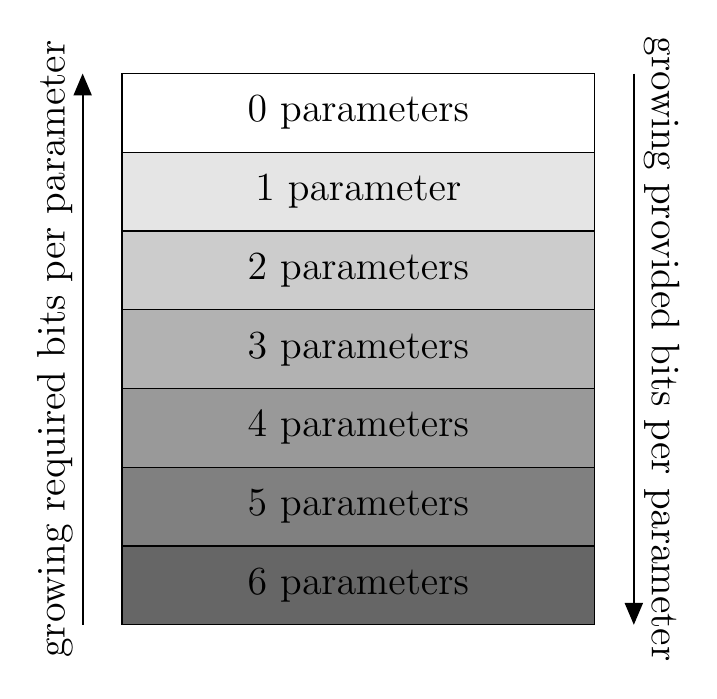
\begin{tikzpicture}

%\fill[black!40!white] (0,0) rectangle (9,9);
%\fill[black!30!white] (0,0) rectangle (7,7);
%\fill[black!20!white] (0,0) rectangle (4,4);
%\fill[black!10!white] (0,0) rectangle (2,2);
%
%\draw (0,0) --node[anchor=south] {0 params}  (2,0)  -- (2,2) -- (0,2) -- (0,0) ;
%\draw (0,0) -- (2,0) --node[anchor=south] {1 param} (4,0) -- (4,4) -- (0,4) -- (0,0);
%\draw (0,0) --(4,0) --node[anchor=south] {2 ... 5 params} (7,0) -- (7,7) -- (0,7) -- (0,0);
%\draw (0,0) --(7,0) --node[anchor=south] {6 params} (9,0) -- (9,9) -- (0,9) -- (0,0);
%\draw[dashed] (4,4) -- (7,7);


\fill[black!00!white] (0,7) rectangle (6,6);
\fill[black!10!white] (0,6) rectangle (6,5);
\fill[black!20!white] (0,5) rectangle (6,4);
\fill[black!30!white] (0,4) rectangle (6,3);
\fill[black!40!white] (0,3) rectangle (6,2);
\fill[black!50!white] (0,2) rectangle (6,1);
\fill[black!60!white] (0,1) rectangle (6,0);


\draw[-triangle 45, thick] (-0.5,0) -- node[sloped, anchor=center, above] {\Large{growing required bits per parameter}} (-0.5,7);
\draw[-triangle 45, thick] (6.5,7) -- node[sloped, anchor=center, above] {\Large{growing provided bits per parameter}} (6.5,0);

\draw (0,7) rectangle node[anchor=center] {\Large{0 parameters}} (6,6);

\draw (0,6) rectangle node[anchor=center] {\Large{1 parameter}}  (6,5);

\draw (0,5) rectangle node[anchor=center] {\Large{2 parameters}} (6,4);

\draw (0,4) rectangle node[anchor=center] {\Large{3 parameters}} (6,3);

\draw (0,3) rectangle node[anchor=center] {\Large{4 parameters}} (6,2);

\draw (0,2) rectangle node[anchor=center] {\Large{5 parameters}} (6,1);

\draw (0,1) rectangle node[anchor=center] {\Large{6 parameters}} (6,0);


\end{tikzpicture}
}
\caption{\emph{Count} policy classification schema for call-sites and call-targets.}
\label{fig:COUNTschema}
\end{figure}


\end{document}
